% mn2esample.tex
%
% v2.1 released 22nd May 2002 (G. Hutton)
%
% The mnsample.tex file has been amended to highlight
% the proper use of LaTeX2e code with the class file
% and using natbib cross-referencing. These changes
% do not reflect the original paper by A. V. Raveendran.
%
% Previous versions of this sample document were
% compatible with the LaTeX 2.09 style file mn.sty
% v1.2 released 5th September 1994 (M. Reed)
% v1.1 released 18th July 1994
% v1.0 released 28th January 1994

\documentclass[useAMS,usenatbib]{mn2e}

% If your system does not have the AMS fonts version 2.0 installed, then
% remove the useAMS option.
%
% useAMS allows you to obtain upright Greek characters.
% e.g. \umu, \upi etc.  See the section on "Upright Greek characters" in
% this guide for further information.
%
% If you are using AMS 2.0 fonts, bold math letters/symbols are available
% at a larger range of sizes for NFSS release 1 and 2 (using \boldmath or
% preferably \bmath).
%
% The usenatbib command allows the use of Patrick Daly's natbib.sty for
% cross-referencing.
%
% If you wish to typeset the paper in Times font (if you do not have the
% PostScript Type 1 Computer Modern fonts you will need to do this to get
% smoother fonts in a PDF file) then uncomment the next line
% \usepackage{Times}

%%%%% AUTHORS - PLACE YOUR OWN MACROS HERE %%%%%
\usepackage{subfigure}
\usepackage{amsmath}	% Advanced maths commands
\usepackage{amssymb}	% Extra maths symbols
\usepackage{graphicx}
%\usepackage{algorithm}
%\usepackage[noend]{algpseudocode}
\usepackage{mathrsfs}
\usepackage{url}

\newcommand{\bz}{\bmath{z}}
\newcommand{\bs}{\bmath{s}}
\newcommand{\bA}{\bmath{A}}
\newcommand{\bB}{\bmath{B}}
\newcommand{\bC}{\bmath{C}}
\newcommand{\bE}{\bmath{E}}
\newcommand{\bF}{\bmath{F}}
\newcommand{\bG}{\bmath{G}}
\newcommand{\br}{\bmath{r}}
\newcommand{\bg}{\bmath{g}}
\newcommand{\bd}{\bmath{d}}
\newcommand{\bv}{\bmath{v}}
\newcommand{\bu}{\bmath{u}}
\newcommand{\bn}{\bmath{n}}
\newcommand{\by}{\bmath{y}}
\newcommand{\bJ}{\bmath{J}}
\newcommand{\bD}{\bmath{D}}
\newcommand{\bH}{\bmath{H}}
\newcommand{\bN}{\bmath{N}}
\newcommand{\bM}{\bmath{M}}
\newcommand{\bO}{\bmath{O}}
\newcommand{\bP}{\bmath{P}}
\newcommand{\bQ}{\bmath{Q}}
\newcommand{\bR}{\bmath{R}}
\newcommand{\bI}{\bmath{I}}
\newcommand{\ba}{\bmath{a}}
\newcommand{\bb}{\bmath{b}}
\newcommand{\bx}{\bmath{x}}
\newcommand{\bp}{\bmath{p}}
\newcommand{\bmJ}{\bmath{\mathcal{J}}}
\newcommand{\bmH}{\bmath{\mathcal{H}}}
\newcommand{\bzero}{\bmath{0}}
\newcommand{\bone}{\bmath{1}}
%\newcommand{\bvarrho}{\bmath{\varrho}}
%\newcommand{\bnu}{\bmath{\nu}}
%\newcommand{\bvarphi}{\bmath{\varphi}}
\newcommand{\conj}[1]{\overline{#1}}

\newcommand{\aaps}{A\&AS}
\newcommand{\aap}{A\&A}
\newcommand{\mnras}{MNRAS}
\newcommand{\nat}{Nature}
\newcommand{\apj}{The Astrophysical Journal}
\newcommand{\prd}{Physical Review Letters D}
\newcommand{\physrep}{Phys. Rep.}
\newcommand{\araa}{Annual Review of Astronomy and Astrophysics}
\newcommand{\pasp}{Publications of the Astronomical Society of Pacific}
\newcommand{\procspie}{Proceedings of the SPIE}
\newcommand{\pasa}{Publications of the Astronomical Society of Australia}


%%%%%%%%%%%%%%%%%%%%%%%%%%%%%%%%%%%%%%%%%%%%%%%%

%\title[Complex redundant calibration]{Redundant calibration as a complex optimization problem}
\title[Redundant interferometric calibration as a complex optimization problem]{Redundant calibration as a complex optimization problem}
%\author[T.L.~Grobler et al.]{T.L.~Grobler$^{1}$\thanks{E-mail: email@address (AVR)}, G.~Bernardi$^{1,2}$, Z.S.~Ali$^{3}$?, C.L.~Carilli$^{4,5}$?, J.S.~Dillon$^{3}$?, A.~Liu$^{3}$?, \newauthor
%A.R.~Parsons$^{3,6}$? and O.M.~Smirnov$^{1,2}$?\\
%$^{1}$Department of Physics and Electronics, Rhodes University, PO Box 94, Grahamstown, 6140, South Africa\\
%$^{2}$SKA SA, 3rd Floor, The Park, Park Road, Pinelands, 7405, South Africa\\
%$^{3}$Dept. of Astronomy, University of California, Berkeley, CA 94720, USA\\
%$^{4}$National Radio Astronomy Obs., Socorro NM\\
%$^{5}$Cavendish Lab., Cambridge UK\\
%$^{6}$Radio Astronomy Lab., U. California, Berkeley CA 94720, USA}
\author[T.L.~Grobler et al.]{T.L.~Grobler$^{1,2}$\thanks{E-mail: email@address (AVR)}, G.~Bernardi$^{2,3}$, C.L.~Carilli$^{4,5}$, J.S.~Kenyon$^{2}$, A.R.~Parsons$^{6,7}$? \newauthor and O.M.~Smirnov$^{2,3}$\\
$^{1}$Dept of Mathematical Sciences, Computer Science Division, Stellenbosch University, Private Bag X1, 7602 Matieland, South Africa\\
$^{2}$Department of Physics and Electronics, Rhodes University, PO Box 94, Grahamstown, 6140, South Africa\\
$^{3}$SKA SA, 3rd Floor, The Park, Park Road, Pinelands, 7405, South Africa\\
$^{4}$National Radio Astronomy Obs., Socorro NM\\
$^{5}$Cavendish Lab., Cambridge UK\\
$^{6}$Dept. of Astronomy, University of California, Berkeley, CA 94720, USA\\
$^{7}$Radio Astronomy Lab., U. California, Berkeley CA 94720, USA}
\begin{document}

%\date{Accepted 1988 December 15. Received 1988 December 14; in original form 1988 October 11}

\pagerange{\pageref{firstpage}--\pageref{lastpage}} \pubyear{2002}

\maketitle

\label{firstpage}

\begin{abstract}
Observations of the redshifted 21-cm line from the epoch of reionization have recently motivated the construction of low 
frequency radio arrays with highly redundant configurations that provide an alternative calibration strategy - 
''redundant calibration" - and boosts sensitivity on specific spatial scales. In this paper we formulate 
calibration of redundant interferometric arrays as a complex optimization problem \citep[i.e.,][]{Smirnov2015}. 
We then solve this optimization problem via the Levenberg-Marquardt algorithm. This calibration approach is more 
robust to initial conditions than current algorithms and, leveraging on an approximate matrix inversion, allows for further optimization and an efficient implementation (``redundant \textsc{StEfCal}"). We also investigated the use of the preconditioned conjugate gradient method as an alternative optimization strategy, instead of 
an approximate matrix inverse, but found that its computational performance is not competitive with respect to ``redundant \textsc{StEfCal}". The efficient implementation of this new algorithm is made publicly available.
%The construction of new radio interferometers, particularly operating at low frequencies and In this paper we show that instead of splitting our redundant calibration problem into its phase-and-amplitude components (the more traditional approach) we can treat the complex unknown model parameters and their complex conjugates as separate unknowns. We also derive the Levenberg-Maquardt and Gauss-Newton update steps associated with this alternative parameter-and-conjugate framework. We focus more on the Levenberg-Maquardt algorithm in this paper as it exhibits better convergence properties when compared to Gauss-Newton. The Gauss-Newton algorithm is currently the de facto standard that is being used to perform redundant calibration. It is common practice to implement redundant calibration via a hierarchical algorithmic strategy. Using the Levenberg-Maquardt algorithm, therefore, reduces the number of algorithmic layers that are needed to perform redundant calibration. We also compare two previously proposed methods to accelerate redundant calibration, namely the alternating direction implicit method and the preconditioned conjugate gradient method. We found that the alternating direction implicit method outperforms the preconditioned conjugate gradient method. However, the preconditioned conjugate gradient method is more robust as it is more straightforward to adapt to other calibration use cases. We make use of the parameter-and-conjugate framework in this paper, rather than the more traditional amplitude-and-phase approach as it makes it trivial to relate the alternating direction implicit method and the Levenberg-Marquardt algorithm with one another.
\end{abstract}


\begin{keywords}
instrumentation: interferometers -- methods: data analysis -- methods: numerical --techniques: interferometric -- cosmology: observations
\end{keywords}

\section{Introduction}
The quest for the redshifted 21-cm line from the Epoch of Reionization (EoR) is a frontier of modern observational cosmology and has motivated the construction of a series of new interferometric arrays operating at low frequencies over the last decade. EoR measurements are challenging because of the intrinsic faintness of the cosmological signal \citep[see, for instance,][for recent reviews]{Furlanetto2016,McQuinn2016} buried underneath foreground emission which is a few orders of magnitude brighter than the EoR anywhere in the sky \citep[e.g.,][]{Bernardi2009,Bernardi2010,Ghosh2012,Dillon2014,Parsons2014}. 
%and that can be separated by leveraging only on the different spectral properties (citations needed!!!). 
As miscalibrated foreground emission leads to artifacts that can jeopardize the EoR signal \citep[e.g.,][]{grobler2014,barry2016,ewall-wice2016}, an exquisite interferometric calibration is required. Such calibration needs an accurate knowledge of both the sky emission and the instrumental response \citep[e.g.,][]{Smirnov2011c}, unless arrays are deployed in a redundant configuration, i.e. with receiving elements placed on regular grids so that they measure many times the same sky brightness emission. Leveraging on this property, redundancy is a promising path to achieve high accurate interferometric calibration \citep[][]{Noordam1982,Wieringa1992,Pearson1984,Liu2010,Noorishad2012,Marthi2014,Sievers2017}. Moreover, redundant configurations provide a sensitivity boost on a selected sample of spatial scales that can be tuned to be the highest signal--to--noise ratio (SNR) EoR modes \citep[][]{Parsons2012,Dillon2016}. These reasons motivated the design and deploment of EoR arrays in redundant configurations like the MIT-EoR \citep{Zheng2014}, the Precision Array to Probe the Epoch of Reionization \citep[PAPER,][]{Ali2015} and the Hydrogen Epoch of Reionization Array \citep[HERA,][]{deboer2017}. 

In this paper we present a new algorithm to calibrate redundant arrays based on the complex optimization formalism recently introduced by \cite{Smirnov2015}. 
With respect to current algorithms, it is more robust to initial conditions, while remaining comparatively fast. We also show that given certain approximations this new algorithm reduces to the redundant calibration equivalent of the \textsc{StEfCal} algorithm \citep{Salvini2014}.
%In this paper we will refer to this simplified version of the new algorithm as redundant StEfCal. 
We investigate the speed-up that the preconditioned conjugate gradient (PCG) method provides if it is employed by the new algorithm \citep{Liu2010}.
A comparison between the computational complexity of the optimized new algorithm and redundant StEfCal is also performed.

The paper is organized as follows: we review the complex calibration formalism by \citet{Smirnov2015} in Section~\ref{sec:sky_wirtinger}, we extend it to the redundant case in Section~\ref{sec:red_wirtinger}, we present some computational complexity results in Section~\ref{sec:pcg} and we conclude in Section~\ref{sec:conclusions}.

%\section{Skymodel-based Wirtinger Calibration}
%\section{Calibration described through the Wirtinger formalism}
\section{Wirtinger calibration}
\label{sec:sky_wirtinger}

In a radio interferometer, the true sky visibilities $y_{pq}$ measured by a baseline formed by antenna $p$ and $q$ are always ``corrupted" by the non-ideal response of the receiver, which is often incorporated into a single, receiver-based complex number $g$. The observed visibility $d_{pq}$ is therefore given by \citep{ME1,ME2,RRIME1}
\begin{equation}
\label{eq:vis_definition}
d_{pq} = g_{p}\conj{g_q} \, y_{pq} + n_{pq},
\end{equation}
where $\conj{(*)}$ indicates conplex conjugation and $n_{pq}$ is the thermal noise component. 
The real and imaginary components of the thermal noise are normally distributed with a mean of zero and a
standard deviation $\sigma$:
\begin{equation}
\sigma \propto \frac{T_{\textrm{sys}}}{\sqrt{\Delta \nu \tau}},
\end{equation}
where $T_{\textrm{sys}}$ is equal to the system temperature, $\Delta \nu$ is the observational bandwidth and $\tau$ is the integration time per visibility.

Considering the number of visibilities $B$ (i.e. baselines) measured by an array of $N$ elements $B = \frac{N^2-N}{2}$, equation~\ref{eq:vis_definition} can be expressed in the following vector form:
\begin{equation}
\label{eq:vis_linear_definition}
\bd = \bv + \bn, 
\end{equation}
where 
\begin{align}
 \left [ \bd \right]_{\alpha_{pq}} &= d_{pq}, & \left [ \bv \right ]_{\alpha_{pq}} &= v_{pq}=g_p y_{pq} \conj{g_q},\nonumber\\
 \left [ \bn \right ]_{\alpha_{pq}} &= n_{pq}, &  &\label{eq:vec_linear_definitions}
\end{align}
and 
\begin{equation}
\alpha_{pq} =
\begin{cases}
(q-p) + (p-1)\left (N-\frac{1}{2}p \right ) & \textrm{if}~p<q\\
0 & \textrm{otherwise}
\end{cases}.
\end{equation}
The function $\alpha_{pq}$ therefore maps composite antenna indexes to unique single indexes, i.e:
\begin{equation}
\{\alpha_{12},\alpha_{13},\cdots,\alpha_{N-1N}\} = \{1,2,\cdots,B\} 
\end{equation}
The vectors in equation~\ref{eq:vec_linear_definitions} are column vectors of size $B$ (i.e. $p<q$).

Radio interferometric calibration aims to determine the best estimate of $\bg = [g_1,g_2,\cdots,g_N]^T$ in order to correct the data and, following equation~\ref{eq:vis_linear_definition}, can be formulated as a non linear least-squares optimization problem:
\begin{equation}
\label{eq:least_squares}
\min_{\bg} \Lambda(\bg) = \min_{\bg} \|\br\|_F^2 = \min_{\bg} \|\bd - \bv(\bg)\|_F^2, 
\end{equation}
where $\Lambda$ is the objective function, $\br$ is the residual vector and $\|\cdot\|_F$ denotes the Frobenius norm. In standard interferometric calibration, $y_{pq}$ is assumed to be known at some level, for instance through the observation of previously known calibration sources. The knowledge of $y_{pq}$ is often named ``sky model".

The gradient-based minimization algorithms that are generally used to solve non-linear least-squares problems are generally solved by using gradient-based minimization algorithms (i.e. Gauss--Newton -- GN -- or Levenberg--Marquardt -- LM) that require the model ($\bv$ in equation~\ref{eq:least_squares}) to be differentiable towards each parameter. 
When the least squares problem is complex, it becomes less straightforward to apply these gradient-based minimization methods, as
many complex functions are not differentiable if the classic notion of differentiation is used, i.e. $\frac{\partial \conj{z}}{\partial z}$ does not exist if $z \in \mathbb{C}$.

In order to circumvent the differentiability conundrum associated with complex least squares problems, standard interferometric calibration divides the complex optimization problem into its real and imaginary parts and solves for the real and imaginary parts of the unknown model parameters separately. \citet{Smirnov2015} showed, however, that this approach is not needed if complex calculus \citep{Wirtinger1927} is directly adopted. The Wirtinger derivatives are defined as:
\begin{align}
\label{eq:wir}
\frac{\partial}{\partial z} &= \frac{1}{2}\left ( \frac{\partial}{\partial x} -  i \frac{\partial}{\partial y} \right ),&\frac{\partial}{\partial \conj{z}} &= \frac{1}{2}\left ( \frac{\partial}{\partial x} +  i \frac{\partial}{\partial y} \right ), 
\end{align}
which lead to the following relations:
\begin{align}
\label{eq:wir_z}
\frac{\partial z}{\partial z} & = 1, & \frac{\partial \conj{z}}{\partial z}&=0, & \frac{\partial z}{\partial \conj{z}} & = 0, & \frac{\partial \conj{z}}{\partial \conj{z}}&=1.
\end{align}
If the gradient operator is defined using equation~\ref{eq:wir}, the model $\bv$ now becomes analytic in both $\bg$ and $\conj{\bg}$ and equation \ref{eq:wir_z} can be used to derive the complex variants of the real-valued GN and LM algorithms. In the complex GN and LM algorithms, complex parameters and their conjugates are treated as separate variables.

Assuming that $y_{pq}$ is known, equation~\ref{eq:least_squares} is recast as \citep{Smirnov2015}:
\begin{equation}
\label{eq:least_squares_augmented}
\min_{\breve{\bg}} \Lambda(\breve{\bg}) = \min_{\breve{\bg}} \|\breve{\br}\|_F^2 = \min_{\breve{\bg}} \|\breve{\bd} - \breve{\bv}(\breve{\bg})\|_F^2, 
\end{equation} 
where $\breve{\br} = [\br^T,\conj{\br}^T]^T$, $\breve{\bd} = [\bd^T,\conj{\bd}^T]^T$, $\breve{\bv} = [\bv^T,\conj{\bv}^T]^T$ and $\breve{\bg} = [\bg^T,\conj{\bg}^T]^T$.

The complex GN update is therefore defined as:
\begin{equation}
\label{eq:GN_update_skymodel}
 \Delta \breve{\bg} = (\bJ^H\bJ)^{-1}\bJ^H\breve{\br},
\end{equation}
with 
\begin{equation}
\label{eq:Jacobian_skymodel}
\bJ = \begin{bmatrix}
       \bmJ & \bmJ^*\\
       \conj{\bmJ}^* & \conj{\bmJ} 
      \end{bmatrix},
\end{equation}
and
\begin{align}
\label{eq:jac_entries}
[\bmJ]_{\alpha_{pq},i} &= \frac{\partial v_{pq}}{\partial g_i}, & [\bmJ^*]_{\alpha_{pq},i} &= \frac{\partial v_{pq}}{\partial \conj{g}_i}. 
\end{align}

The complex LM update is very similar, the major difference being a damping factor $\lambda$ is introduced:
\begin{equation}
\label{eq:LM_update_skymodel}
\Delta \breve{\bg} = (\bJ^H\bJ + \lambda\bD)^{-1}\bJ^H\breve{\br},
\end{equation}
where $\bD=\bI\odot\bJ^H\bJ$. In this paper, the identity matrix is denoted by $\bI$. Moreover, the Hadamard product and the Hermition transpose are denoted by $\odot$ and $(\cdot)^H$. Note the use of the Wirtinger derivatives in equation~\ref{eq:jac_entries}.
We will refer to $\bJ^H\bJ$ as the Hessian matrix $\bH$ and to $\bJ^H\bJ + \lambda\bD$ as the modified Hessian matrix $\bmH$ throughout this paper. 

Equation~\ref{eq:GN_update_skymodel} or~\ref{eq:LM_update_skymodel} can now be used iteratively to update the parameter vector $\breve{\bg}$:
\begin{equation}
\label{eq:update_skymodel}
\breve{\bg}_{k+1} = \breve{\bg}_{k} + \Delta \breve{\bg}_{k},
\end{equation}
until convergence is reached.

In the case of the GN algorithm, the parameter update step simplifies and becomes \citep{Smirnov2015}
\begin{equation}
\label{eq:one_half}
\breve{\bg}_{k+1} = (\bJ^H\bJ)^{-1}\bJ^H\breve{\bd} + \frac{1}{2}\breve{\bg}_{k}. 
\end{equation}


\citet{Smirnov2015} realized that the diagonal entries of the Hessian matrix $\bH$ are much more significant than its off-diagonal entries, i.e. $\bH$ is nearly diagonal. By approximating $\bH$ by its diagonal and substituting the approximate Hessian matrix the LM parameter update step becomes \citep{Smirnov2015}:
\begin{align}
\breve{\bg}_{k+1} &\approx \frac{1}{1+\lambda}\widetilde{\bH}^{-1}\bJ^H\breve{\bd} + \frac{\lambda}{1+\lambda} \breve{\bg}_k, \nonumber \\
 &= \alpha \widetilde{\bH}^{-1}\bJ^H\breve{\bd} + (1-\alpha)\breve{\bg}_k, 
\label{eq:stef_alpha}  
\end{align}
where $\alpha = \frac{1}{1+\lambda}$. Note that equation~\ref{eq:one_half} and equation~\ref{eq:stef_alpha} are   
not dependent on $\breve{\br}$. 

Interestingly enough, if $\lambda = 0$ we obtain the odd parameter update step of \textsc{StEfCal}\footnote{$k\in\{0,2,\cdots\}$}, and if $\lambda=1$ (which corresponds
to $\alpha=\frac{1}{2}$) we obtain the even parameter update step of \textsc{StEfCal}\footnote{$k\in\{1,3,\cdots\}$} \citep[\textsc{StEfCal},][]{Mitchell:MWA-cal,Salvini2014}. In the \textsc{StEfCal} algorithm, the measurement equation, equation~\ref{eq:vis_definition}, is linearized by assuming that the gains are known, but that their conjugates are not. Under this assumption, the system of equations become linear and the conjugates of the gains can be obtained straightforwardly. Starting from the latest value of the gain conjugates, an updated estimate of the gains can be obtained and the succession continues until convergence is reached.
Alternating between solving and fixing different sets of parameters (which is exactly what \textsc{StEfCal} does) is in general referred to 
as the alternating direction implicit method (ADI). The \textsc{StEfCal} algorithm reduces the computational complexity of calibration from $O(N^3)$ to $O(N^2)$.

\section{Redundant Wirtinger Calibration}
\label{sec:red_wirtinger}
Interferometric baselines are named redundant when they sample the exact same visibilities in the $uv$-plane, i.e. if baseline $pq$ and $rs$ are redundant then $y_{pq} = y_{rs}$. It is convenient to group redundant visibilities together and label each group using a single index rather than using their antenna pairs as in equation~\ref{eq:vis_definition}. We introduce a function $\phi_{pq}$ that maps the antenna pair associated with a specific baseline to the single group index of the redundant baseline group that includes the baseline in question, i.e. if baseline $pq$ and $rs$ are redundant then $\phi_{pq} = \phi_{rs}$. The function $\phi_{pq}$ is not symmetric as $\phi_{pq} = 0$ if $p \geq q$. Equation~\ref{eq:vis_definition} can be re-written for a redundant array as:
\begin{equation}
\label{eq:vis_red}
d_{pq} = g_{p}\conj{g_q}y_{\phi_{pq}} + n_{pq},
\end{equation}
with the same vector form as equation~\ref{eq:vis_linear_definition} if
\begin{align}
 \left [ \bd \right]_{\alpha_{pq}} &= d_{pq}, & \left [ \bv \right ]_{\alpha_{pq}} &= v_{pq}=g_p y_{\phi_{pq}} \conj{g_q},\nonumber\\
 \left [ \bn \right ]_{\alpha_{pq}} &= n_{pq}, &  &\label{eq:vec_definitions}
\end{align}
where the vectors in Equation~\ref{eq:vec_definitions} are column vectors of size $B$ (i.e. $p<q$).

We also introduce the following symmetric variant of $\phi_{pq}$:
\begin{equation}
\zeta_{pq} = 
\begin{cases}
\phi_{pq}~\textrm{if}~p \leq q\\
\phi_{qp}~\textrm{if}~p>q
\end{cases},
\end{equation} 
and we will refer to $\zeta_{pq}$ as the symmetric geometric function.
It is possible to construct a simple analytic expression for $\zeta_{pq}$ for an east-west regular array, i.e. $\zeta_{pq} = |q-p|$. It becomes, however, increasingly difficult to construct analytic expressions of $\zeta_{pq}$ for more complicated array layouts. The empirically constructed symmetric geometry functions of three different redundant layouts are displayed in Figure~\ref{fig:geometry_function}. We denote the range of $\zeta_{pq}$ with $\mathcal{R}(\zeta_{pq})$. The maximal element that $\zeta_{pq}$ can ascertain is denoted by $L$ and can be interpreted as the maximal number of unique redundant baseline groups which can be formed for a given array layout. 

\begin{figure*}
\centering
\subfigure[Hexagonal layout]
{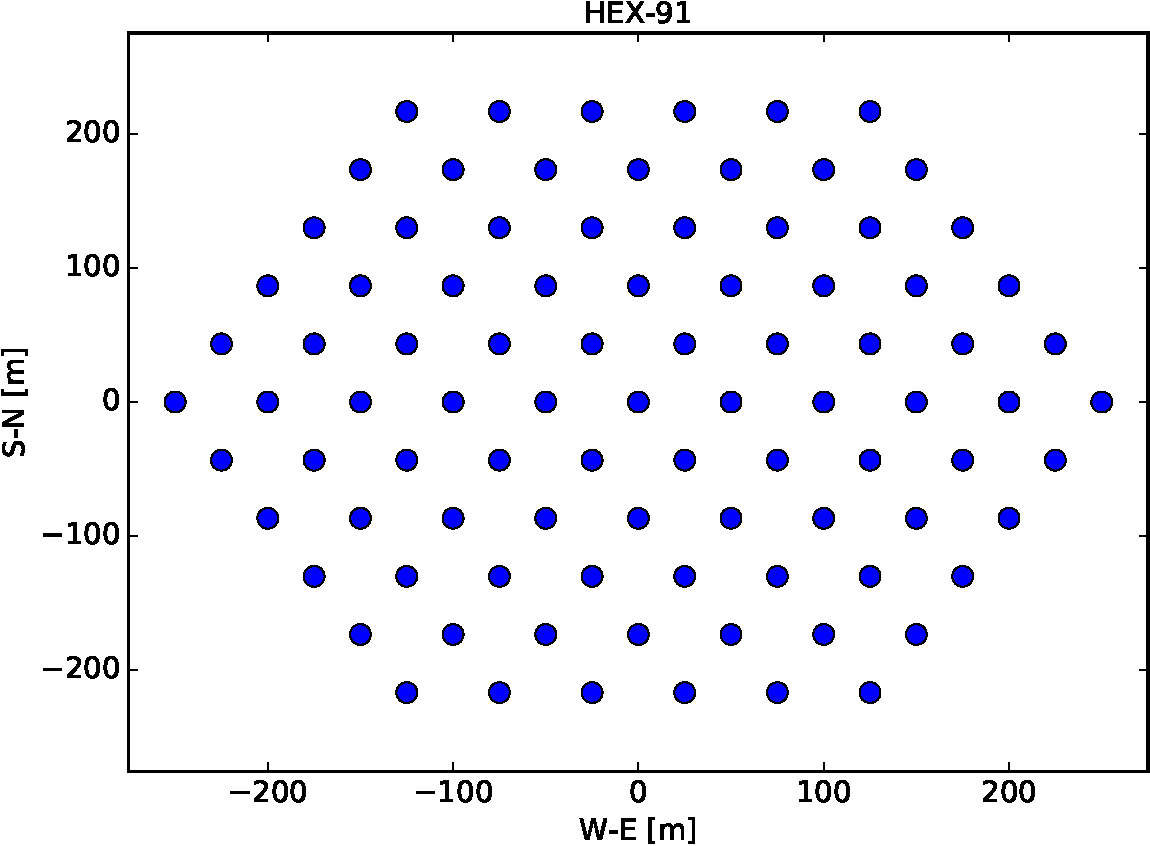
\includegraphics[width=0.32\textwidth]{./HEX_lay.pdf}\label{fig:HEX_lay}}
\subfigure[Square layout]
{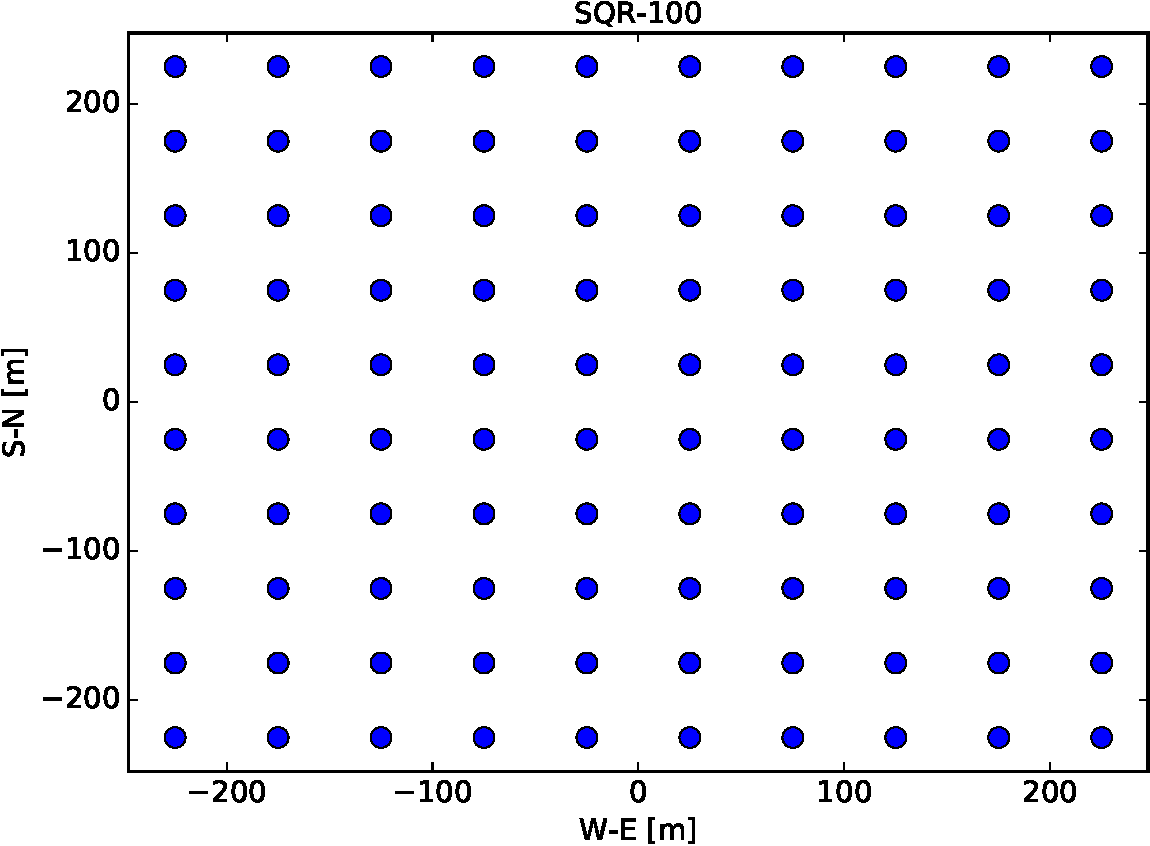
\includegraphics[width=0.32\textwidth]{./SQR_lay.pdf}\label{fig:SQR_lay}}
\subfigure[Regular east-west layout]
{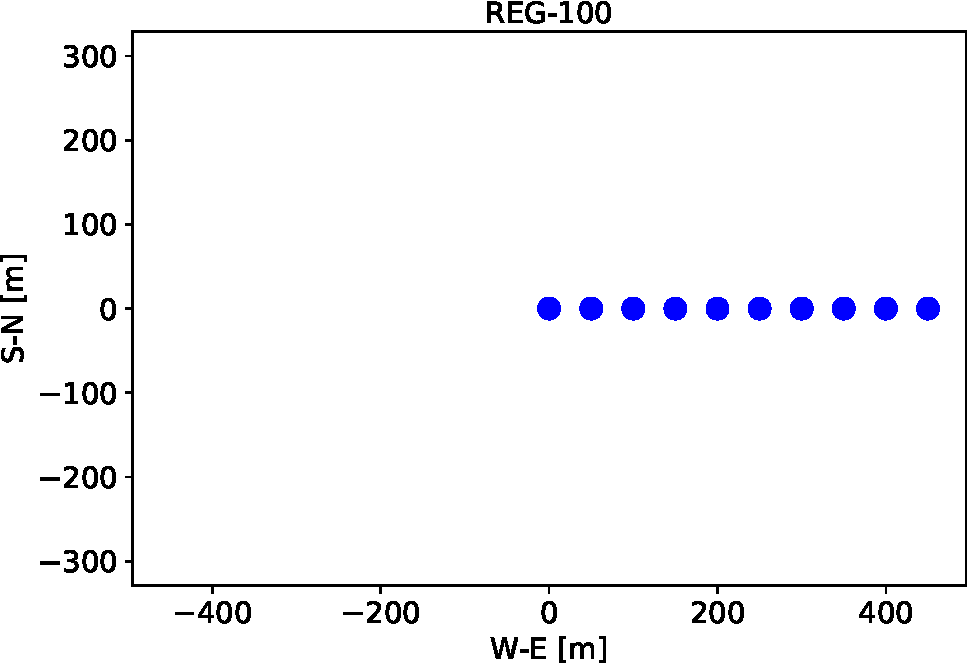
\includegraphics[width=0.32\textwidth]{./REG_lay.pdf}\label{fig:REG_lay}}

\subfigure[Hexagonal: $\zeta_{pq}$]
{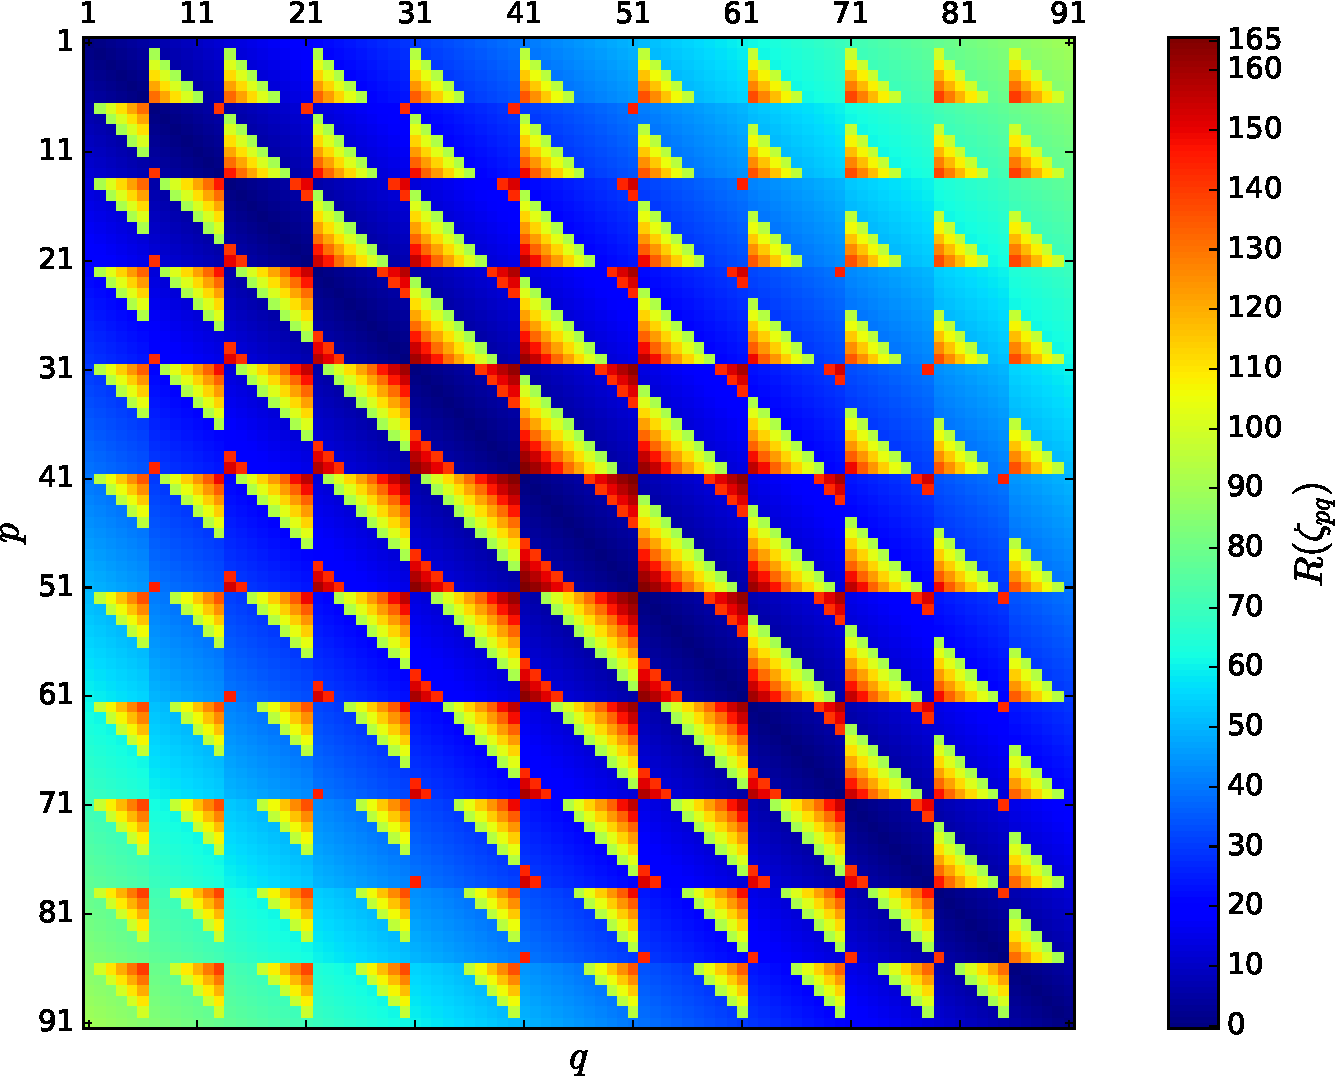
\includegraphics[width=0.33\textwidth]{./HEX_phi.pdf}\label{fig:HEX_phi}}
\subfigure[Square: $\zeta_{pq}$]
{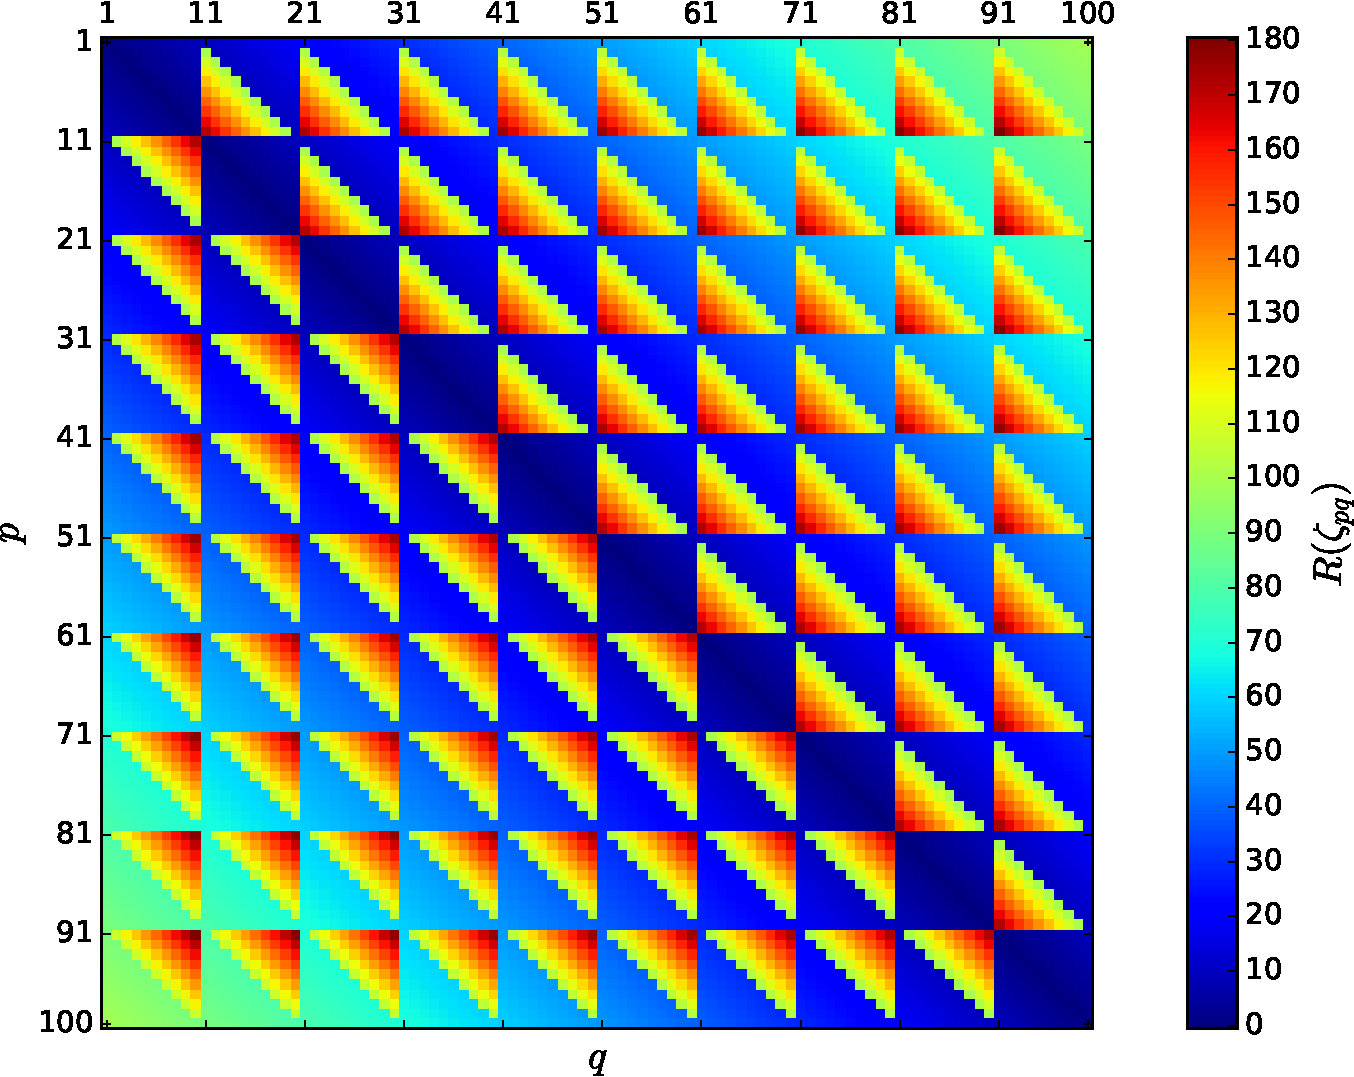
\includegraphics[width=0.33\textwidth]{./SQR_phi.pdf}\label{fig:SQR_phi}}
\subfigure[Regular east-west: $\zeta_{pq}$]
{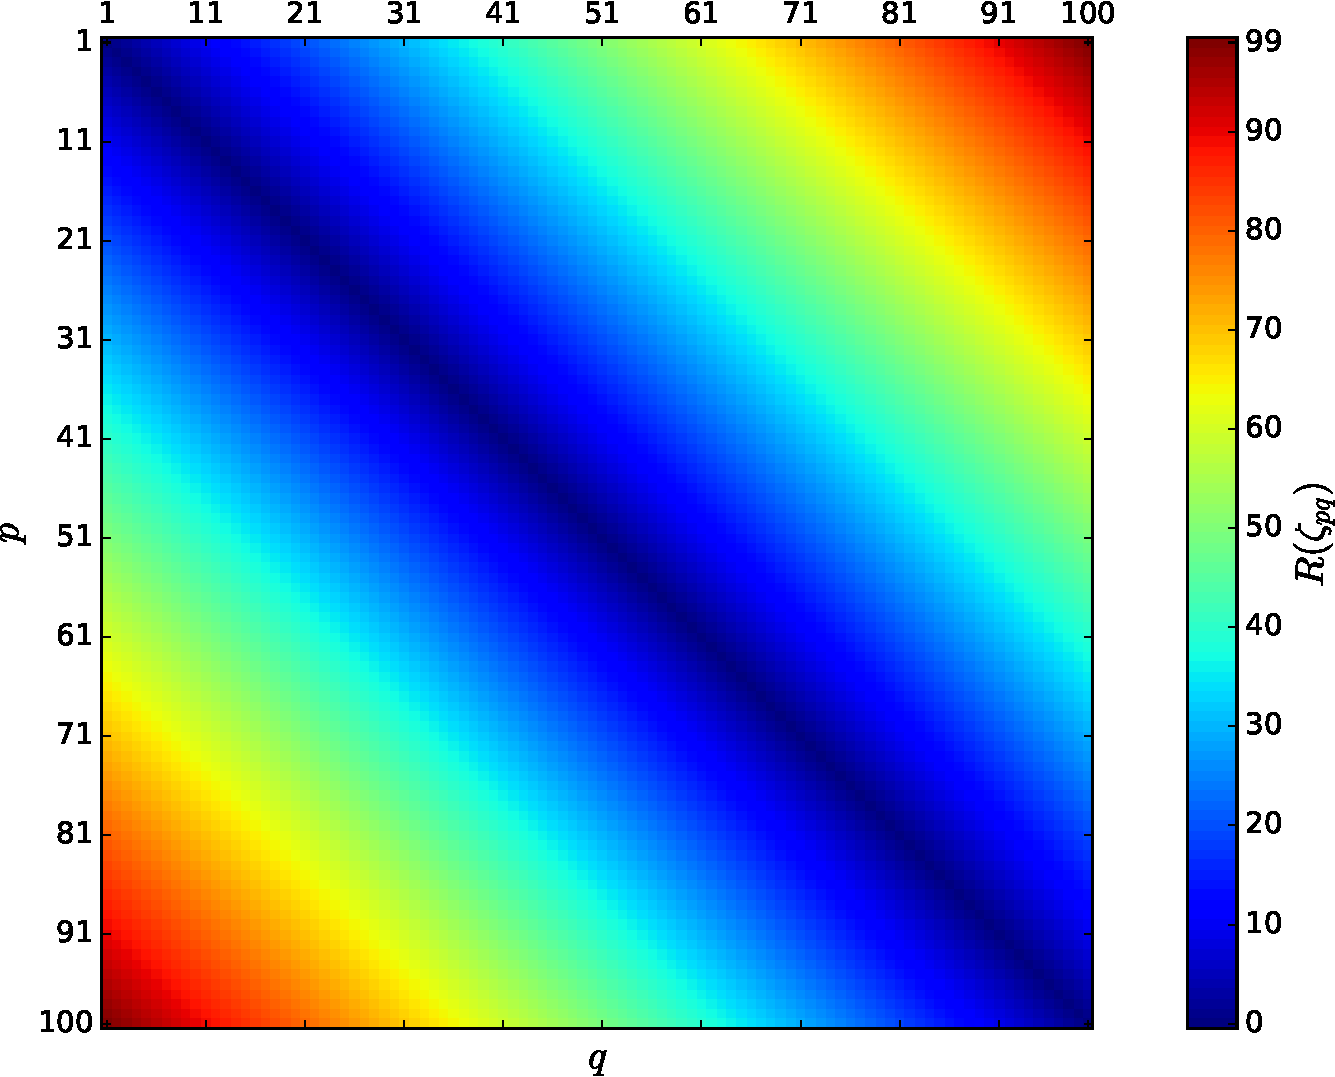
\includegraphics[width=0.33\textwidth]{./REG_phi.pdf}\label{fig:REG_phi}}
\caption{Three different redundant antenna layouts: hexagonal (top left), square (top middle) and regular east-west (top right) with their respective symmetric redundancy geometry functions $\zeta_{pq}$ (bottom panels). We used 91 antennas to construct the hexagonal layout, while 100 antennas were used in the square and east-west layouts. In the case of the east-west layout we only plot the positions of the first ten antennas. The maximal amount of redundant baseline groups $L$ that can be formed for 
the hexagonal, square and east-west layouts are 165, 180 and 99 respectively. The analytic expressions of $L$ for an hexagonal, square and east-west layout is $L = 2N-\frac{1}{2}\sqrt{12N-3}-\frac{1}{2}$,
$L=2N-2\sqrt{N}$ and $L=N-1$.\label{fig:geometry_function}}
\end{figure*}

We can now formulate redundant calibration as a least-squares problem:
\begin{equation}
\label{eq:least_squares_red}
\min_{\bz} \Lambda(\bz) = \min_{\bz} \|\br\|_F^2 = \min_{\bz} \|\bd - \bv(\bz)\|_F^2, 
\end{equation}
where
\begin{align}
 \bg &=[g_1,\cdots,g_N]^T, & \by &= [y_1,\cdots,y_L]^T,\nonumber\\
 \bz &= [\bg^T,\by^T]^T. &  &\label{eq:parm_definitions}
 \end{align}
The number of model parameters to be solved for is now $P = 2(N+L)$, since redundant calibration is a complex problem.

In literature, equation~\ref{eq:least_squares_red} is solved by splitting the problem into its real and imaginary parts. The real and imaginary parts of the unknown parameters are then solved for separately \citep{Wieringa1992,Liu2010,Zheng2014}. 
Currently, the above is achieved by using the real-valued GN algorithm \citep{Kurien2016}. 
We, instead, intend to formulate the redundant calibration problem using Wirtinger calculus and recast equation~\ref{eq:least_squares_red} as
\begin{equation}
\label{eq:least_squares_complex}
\min_{\breve{\bz}} \|\breve{\br}\| = \min_{\breve{\bz}} \|\breve{\bd} - \breve{\bv}(\breve{\bz})\|, 
\end{equation}
where $\breve{\bz} = [\bz^T,\conj{\bz}^T]^T$. 
We derive the complex Jacobian associated with equation~\ref{eq:least_squares_complex} to be:
\begin{equation}
\label{eq:Jacobian}
\bJ = \begin{bmatrix}
       \bmJ & \bmJ^*\\
       \conj{\bmJ}^* & \conj{\bmJ} 
      \end{bmatrix},
\end{equation}
where 
\begin{equation}
[\bmJ]_{\alpha_{pq},i} = \begin{cases} 
     \frac{\partial v_{pq}}{\partial g_i} & \textrm{if}~i\leq N \\
     \frac{\partial v_{pq}}{\partial y_{i-N}} & \textrm{otherwise}  
\end{cases}, %, & \bmJ^* &= \frac{\partial \bv}{\partial \conj{\bz}}. 
\end{equation}
and
\begin{equation}
[\bmJ^*]_{\alpha_{pq},i} = \begin{cases} 
     \frac{\partial v_{pq}}{\partial \conj{g}_i} & \textrm{if}~i\leq N \\
     \frac{\partial v_{pq}}{\partial \conj{y}_{i-N}} & \textrm{otherwise}  
\end{cases}. %, & \bmJ^* &= \frac{\partial \bv}{\partial \conj{\bz}}. 
\end{equation}
We can now calculate the GN and LM updates to be 
\begin{equation}
\label{eq:GN_update}
\Delta \breve{\bz} = (\bJ^H\bJ)^{-1}\bJ^H\breve{\br}
\end{equation}
and 
\begin{equation}
\label{eq:LM_update}
\Delta \breve{\bz} = (\bJ^H\bJ + \lambda\bD)^{-1}\bJ^H\breve{\br},
\end{equation}
respectively. As in Section~\ref{sec:sky_wirtinger}, equation~\ref{eq:GN_update} can be used to iteratively update our parameter vector:
\begin{equation}
\label{eq:update}
\breve{\bz}_{k+1} = \breve{\bz}_{k} + \Delta \breve{\bz}_{k}. 
\end{equation}
The analytic expressions for $\bJ$, $\bH$ and $\bJ^H\breve{\br}$ can be found in Appendix~\ref{sec:analytic}.
Appendix~\ref{sec:analytic} also contain two useful identities, involving $\bJ$ and $\bH$. 

In the case of the GN algorithm we can simplify equation~\ref{eq:update} even further. Replacing $\breve{\br}$ with $\breve{\bd}-\breve{\bv}$ in equation~\ref{eq:GN_update} results in
\begin{equation}
\label{eq:temp_GN_eq}
\Delta \breve{\bz} = (\bJ^H\bJ)^{-1}\bJ^H(\breve{\bd}-\breve{\bv}), 
\end{equation}
If we substitute the first identity of equation~\ref{eq:identities} into equation~\ref{eq:temp_GN_eq} and we simplify the 
result we obtain 
\begin{equation}
\label{eq:one_thrid}
\Delta \breve{\bz} = (\bJ^H\bJ)^{-1}\bJ^H\breve{\bd}-\frac{1}{3}\breve{\bz}.
\end{equation}
If we use the above simplified update in equation~\ref{eq:update} it reduces to
\begin{equation}
\label{eq:two_thrids}
\breve{\bz}_{k+1} = (\bJ^H\bJ)^{-1}\bJ^H\breve{\bd} + \frac{2}{3}\breve{\bz}_{k}. 
\end{equation}
Equation~\ref{eq:two_thrids} is the redundant equivalent of equation~\ref{eq:one_half} and it shows us that in the case of redundant calibration we can calculate the GN parameter update step without calculating the residual.  

\begin{figure*}
\centering
\subfigure[Regular layout]{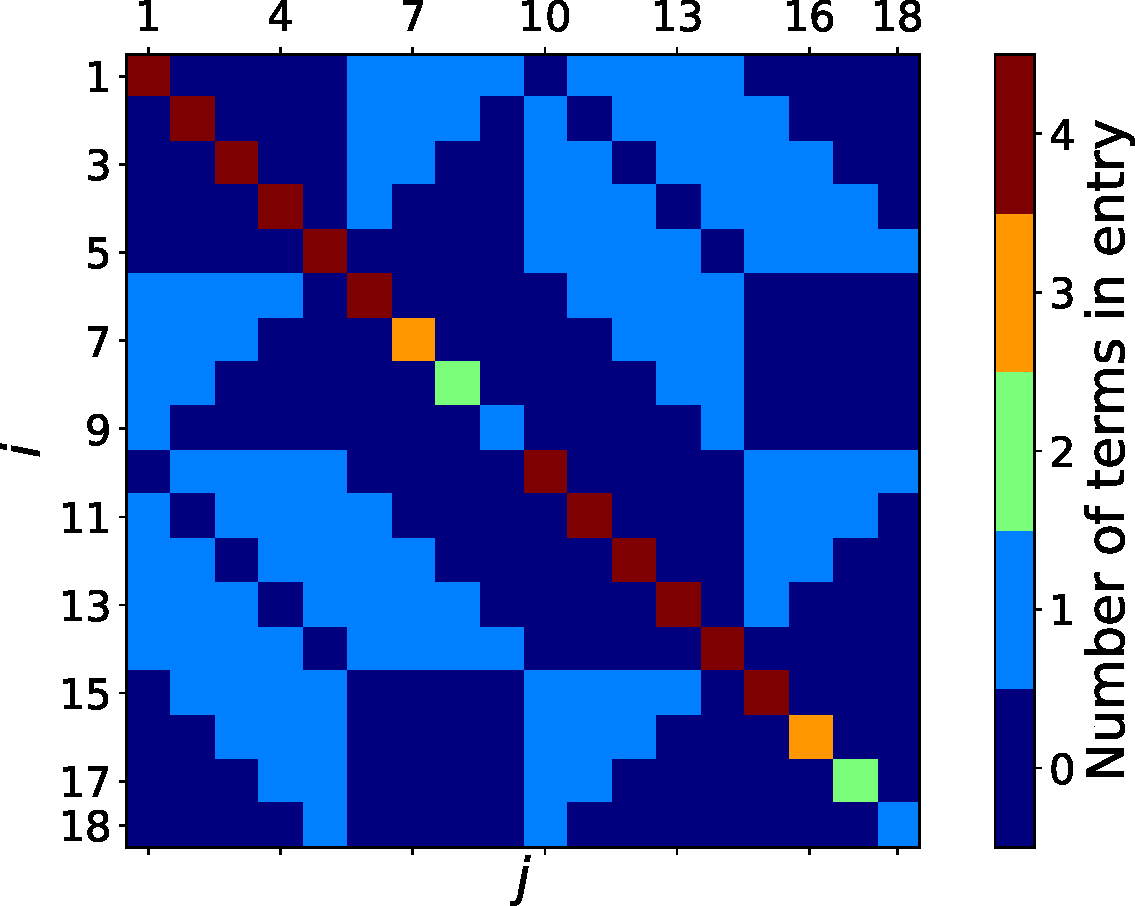
\includegraphics[width=0.47\textwidth]{./reg_hessian.pdf}\label{fig:hessian_reg}}
% V_R_3.pdf: 585x441 pixel, 72dpi, 20.64x15.56 cm, bb=0 0 585 441
\subfigure[Hexagonal layout]{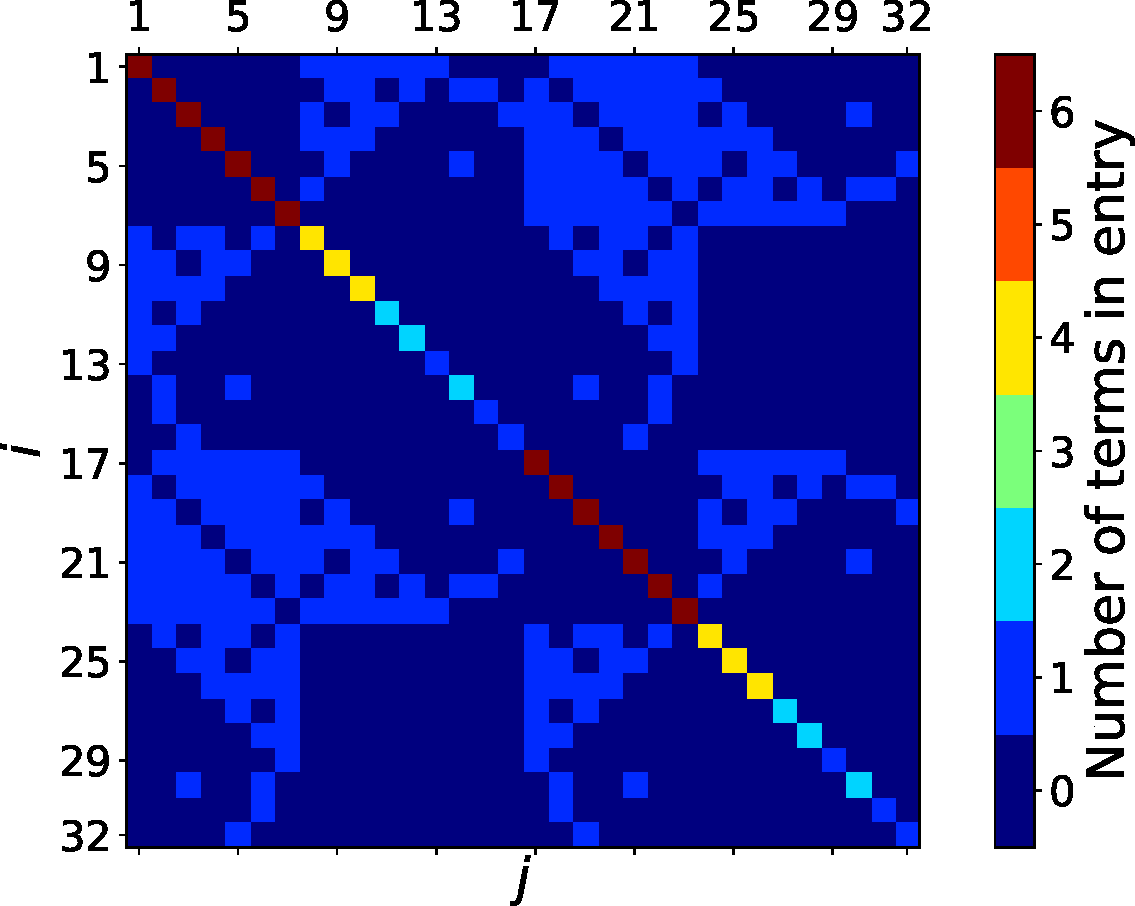
\includegraphics[width=0.47\textwidth]{./hex_hessian.pdf}\label{fig:hessian_hex}}
\caption{The number of analytic terms out of which the entries of the Hessian $\bH$ consist for two different geometric layouts, namely a regular east-west grid with $N = 5$ (left panel) and 
a hexagonal grid with $N = 7$. The diagonal entries of these two Hessians are clearly more significant than their off-diagonal entries. Moreover, these two Hessians also 
contain many zero-entries. Note that the locations of the zero-entries are dependent on the geometry of the array layout.
\label{fig:hessian}} 
\end{figure*}

Figure~\ref{fig:hessian} shows that the Hessian matrix $\bH$ is nearly diagonal and sparse for both a regular and hexagonal layout considered. We therefore follow the approach of \citet{Smirnov2015} and approximate the Hessian matrix $\bH$ with its diagonal. If we substitute $\bJ^H\bJ$ with $\widetilde{\bH}=\bH\odot\bI$ and replace $\breve{\br}$ with $\breve{\bd} - \breve{\bv}$ in equation~\ref{eq:GN_update} we obtain:
\begin{equation}
\label{eq:appr_GN}
 \Delta \breve{\bz} \approx \widetilde{\bH}^{-1}\bJ^H(\breve{\bd}-\breve{\bv})
\end{equation}
Utilizing the second identity in equation~\ref{eq:identities} allows us to simplify equation~\ref{eq:appr_GN} to
\begin{equation}
  \Delta \breve{\bz} \approx \widetilde{\bH}^{-1}\bJ^H\breve{\bd}-\breve{\bz},
\end{equation}
which leads to
\begin{equation}
 \breve{\bz}_{k+1} \approx \widetilde{\bH}^{-1}\bJ^H\breve{\bd}.
\end{equation}
We obtain a similar result if we repeat the above procedure, only in this case we use equation~\ref{eq:LM_update} instead. Thus,
\begin{align}
\breve{\bz}_{k+1} &\approx \frac{1}{1+\lambda}\widetilde{\bH}^{-1}\bJ^H\breve{\bd} + \frac{\lambda}{1+\lambda} \breve{\bz}_k,\label{eq:lambda}\\
 &= \alpha \widetilde{\bH}^{-1}\bJ^H\breve{\bd} + (1-\alpha)\breve{\bz}_k. \label{eq:alpha}  
\end{align}
The analytic expression of $\bJ^H\breve{\bd}$ will be very similar to the analytic 
expression of $\bJ^H\breve{\br}$, the only difference being that in equation~\ref{eq:ab} the letter $r$ would be replaced by a $d$. If we substitute the analytic expression
of $\bJ^H\breve{\bd}$ and $\widetilde{\bH}^{-1}$ (which can easily be constructed using Appendix~\ref{sec:analytic}) into equation~\ref{eq:alpha} we obtain the following two update rules:
\begin{equation}
\label{eq:g_update}
g_{i}^{k+1} = \alpha \frac{\sum_{j\neq i} g_j^k \widetilde{y}_{ij}^{~\!\!k} d_{ij}}{\sum_{j\neq i} |g_j^k|^2|y_{\zeta_{ij}}^k|^2} + (1-\alpha) g_i^k, 
\end{equation}
and
\begin{equation}
\label{eq:y_update}
y_{i}^{k+1} = \alpha \frac{\sum_{rs \in \mathcal{RS}_i} \conj{g}_r^k g_s^k d_{rs}}{\sum_{rs \in \mathcal{RS}_i}|g_r^k|^2|g_s^k|^2} + (1-\alpha) y_i^k. 
\end{equation}
The the index set $\mathcal{RS}_i$ and the quantity $\widetilde{y}_{ij}$ is defined in equation~\ref{eq:RS} and equation~\ref{eq:y_tilde}, respectively. 
The computational complexity of inverting $\widetilde{\bH}$ is $O(P)$. We note that equation~\ref{eq:g_update} is the gain estimator associated with \textsc{StEfCal}.

Equation~\ref{eq:g_update} and~\ref{eq:y_update} were obtained by \citet{Marthi2014} by taking the derivative of the objective function $\Lambda$ relative to the elements of $\bg$ and $\by$, setting the intermediate results to zero and then solving for the unknown parameters (i.e. using the gradient descent algorithm). 
We note that their derivation is less general. The LM algorithm has better convergence properties than gradient descent and 
encompasses the gradient descent algorithm as a special case. In Appendix~\ref{sec:red_stef_ADI} we show that equation~\ref{eq:g_update} and~\ref{eq:y_update} can also be derived using the ADI method. 
For this reason, we refer to the code implementation of the pseudo LM calibration scheme, derived above (equation~\ref{eq:g_update} and~\ref{eq:y_update}), as redundant \textsc{StEfCal}, throughout the rest of the paper.

The choice of the $\alpha$ parameter is somewhat unconstrained. In this paper we chose $\alpha$ by adopting the same strategy that is used by \textsc{StEfCal} and \citet{Marthi2014},
i.e. we chose $\alpha$ to be equal to a $\frac{1}{3}$ ($\lambda = 2$). We also carried out simulations to validate this choice.
%In the case of \textsc{StEfCal}, $\alpha = \frac{1}{2}$ (for even iterations), which results in the last term of equation~\ref{eq:one_half} and equation~\ref{eq:stef_alpha} being equal. When $\alpha=\frac{1}{3}$, the last term of equation~\ref{eq:two_thrids} and equation~\ref{eq:alpha} are equal.

We generated a sky model that comprises of 100 flat spectrum sources distributed over a 3$^{\circ}$ by 3$^{\circ}$ sky 
patch centred. The flux density of each source was drawn from a power law distribution with a slope of 2 and the source position drawn from a uniform distribution. 
We also made use of multiple fictitious telescope layouts each one having a hexagonal geometry (see the left upper image of Figure~\ref{fig:geometry_function} for an example layout). The largest hexagonal array that we used has 217 antennas, with a minimum and maximum baseline of of 20~m and 320~m respectively.

We "corrupted" visibilities by applying gain errors (Table~\ref{tab:gain_parm}) and calibrated the corrupted visibilities using redundant \textsc{StEfCal}. Solutions were independently derived for each time-step and channel for five realizations. 

\begin{table*}
\centering
\caption{The gain error models used in this paper. We have used the symbol $x$ here as a proxy as it can either refer to time-slots or channels. We either
performed our simulations over multiple time-slots and one frequency channel or one timeslot and multiple frequencey channels (see Table~\ref{tab:ch_parm}). Moreover, $c$ in the left most column denotes the speed of light.
We adopted a sinusoidal error model as well as phase slope across frequency that mimics a real case of physical delays between different antennas.
It is worth pointing out the following. In the first model, we model a gain error with amplitude around one and an additional phase error. In 
the second model we chose $A$ in such a way that we do not unintentionally produce a zero gain value. For the third model 
the value of $\tau$ was chosen so that the amount of phase wraps that occur across the observing band is restricted to a realistic number.
{\bf (GB: we need a final better description of the models, but we can work this out later).}}
\begin{tabular}{|c c c c|} 
\hline
Number tag & 1 & 2 & 3\\
Model & Sinusoidal: amplitude and phase & Sinusoidal: real and imaginary parts & Linear phase slope \\ [0.5ex] 
\hline\hline
Function & $(A+1)e^{jP}$ & $A\cos(2\pi fx+B)+1.5A+jC\sin(2\pi fx+D)$ & $e^{jP}$ \\ 
\hline
Parameters & $A=a\cos(2\pi fx +b)$  & $f=5$ & $P=\tau x$ \\
 & $P =c \cos(2\pi fx +d)$ & $A,C\sim U[0.5,10]$ & $\tau = \frac{l}{c}$ \\
 & $f=5$ & $B,D\sim U[0,2\pi]$ &  $l\sim U[5,50]$ (m)\\
 & $a\sim U[0.8,0.9]$ &  & \\ 
 & $c\sim U[0.5,5]$ &  &  \\ 
 & $b,d\sim U[0,2\pi]$ &  &  \\ 
\hline
\end{tabular}
\label{tab:gain_parm}
\end{table*}

\begin{table}
\centering
\caption{We generated results using two main setups. We either used one frequency channel and multiple time-slots, or one time-slot and multiple frequency channels. The most important parameters used in realizing these two major setups are presented here. %Note that we refer to the gain error models in the last row of Table~\ref{tab:gain_parm}. 
We chose the observational frequency band of setup 1 to coincide with the HERA array. To broaden the scope of our 
analysis we chose the observational frequency of our second setup to be equal to 1.4~GHz, which is a typical observing frequency of the Westerbork Synthesis Radio Telescope.}
\begin{tabular}{|c c c|} 
\hline
 & Setup 1 & Setup 2\\
\hline
\hline
 Num. channels & 1024 & 1\\
$\nu$-range & 100-200 MHz & 1.4 GHz\\
Num. timeslots & 1 & 50\\
%Hour angle &-1^h & [-1^h,1^h]\\
%Gain error model (Table~\ref{tab:gain_parm}) & 2 & 1\\
%Initial guess: $\bz_0$ & $\bone$ & $\bone$\\
\hline
\end{tabular}
\label{tab:ch_parm}
\end{table}

The simulated visibilities included a noise term. The purpose of which is to produce a certain SNR in the simulated
visibilities. We made use of the following definition of \citep[SNR, ][]{Liu2010,Marthi2014}:  
\begin{equation}
\label{}
\textrm{SNR} = 10\log \left (\frac{<\bv\odot\conj{\bv}>_{\nu,t,pq}}{<\bn\odot\conj{\bn}>_{\nu,t,pq}} \right ), 
\end{equation}
where $<*>_{\nu,t,pq}$ denotes averaging over frequency, time and baseline.

Figure~\ref{fig:prec_error} show the simulation results as a function of SNR and number of antennas. The accuracy of our solutions is quantified through the percentage error
\begin{equation}
\label{eq:beta}
\beta = \frac{\|\bv - \widehat{\bv}\|_F^2}{\|\bv\|_F^2},
\end{equation}
where $\widehat{\bv}$ is the redundant \textsc{StEfCal} parameter estimate.

The error magnitude follows the expected behaviour, i.e., it decreases as a function of SNR and number of antennas $N$. Interestingly, it reduces to a few percent when $N > 120$ for essentially any choice of SNR. 
%\citet{Marthi2014} conducted an even more in depth analysis than the one presented here. They found that the total computational cost of the algorithm associated with redundant StEfCal is $O(P^2)$ and that it approaches the Cram{\'e}r-Rao Bound (CRB) at moderate SNRs. 

\begin{figure}
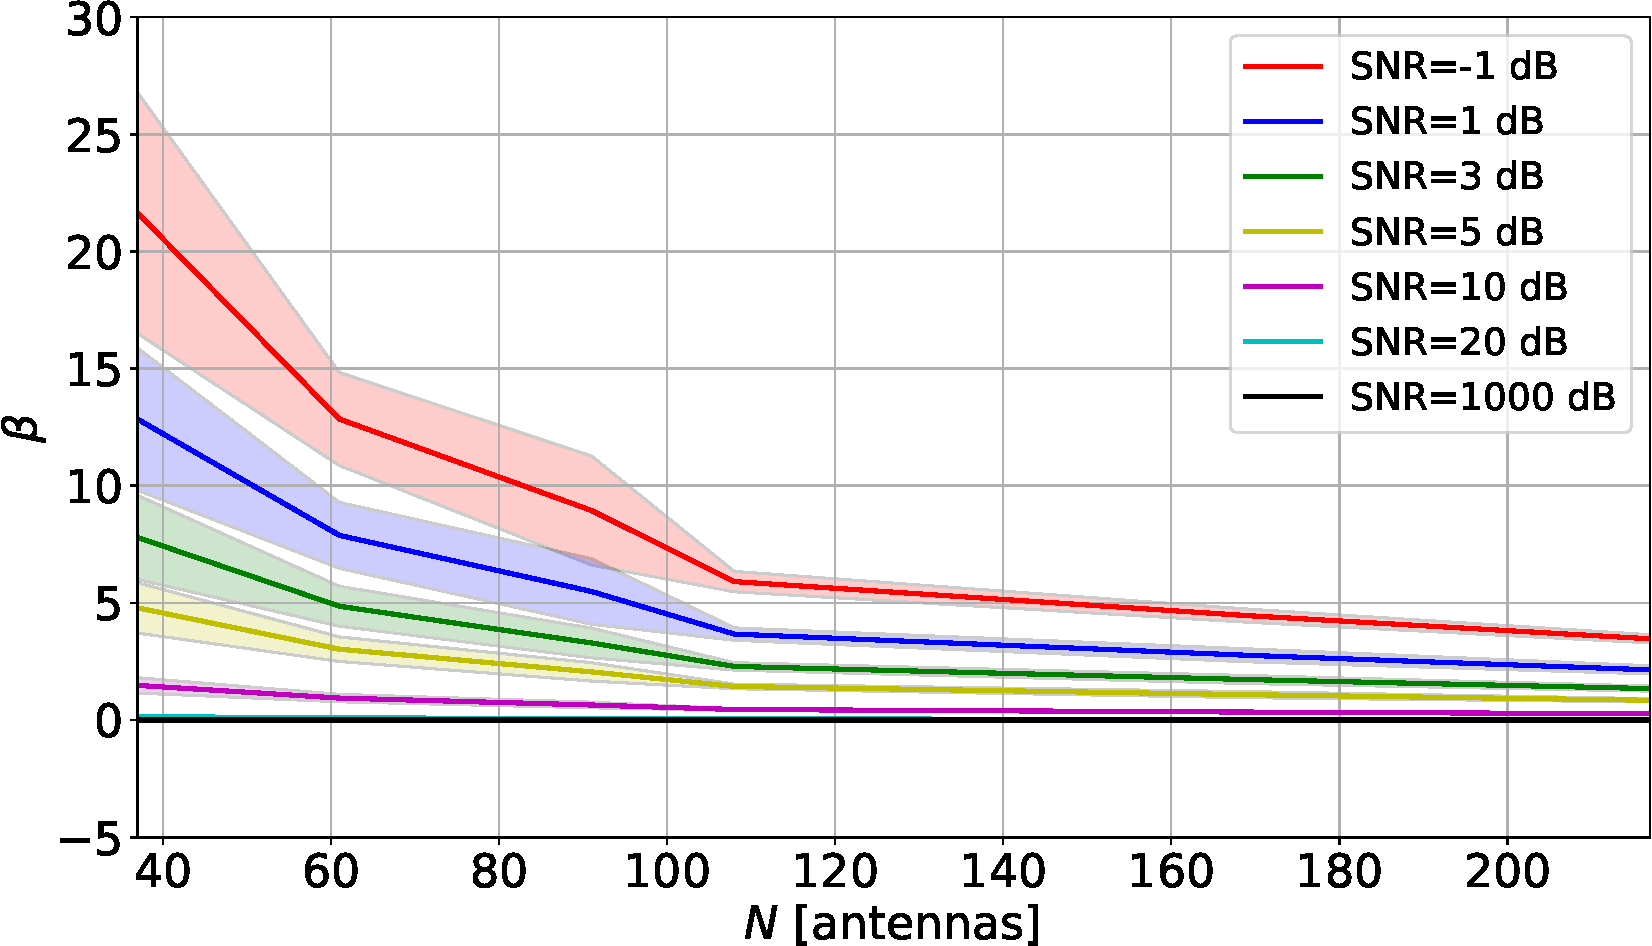
\includegraphics[width=0.47\textwidth]{./prec_error.pdf} 
\caption{We plot the percentage error $\beta$ between the simulated visibilitied and the visibilities solved for by redundant \textsc{StEfCal} for different SNR values as a function of the number of antennas in the array $N$.}
\label{fig:prec_error}
\end{figure}


\section{Preconditioned Conjugate Gradient Method}
\label{sec:pcg}
\citet{Liu2010} suggested that the speed of convergence of redundant calibration could be optimized using the 
conjugate gradient method \citep{Hestenes1952}, which would be computationally advantageous, since the Hessian matrix associated 
with redundant calibration (see Figure~\ref{fig:hessian}) is sparse \citep{Reid1971}. In this section we study the computational complexity
of the conjugate gradient (CG) method when it is used to invert the modified Hessian matrix (see equation~\ref{eq:LM_update}), 
in particular when preconditioning is used (i.e. the PCG method). Interestingly, emperical tests suggests that the unmodified Hessian itself is singular. It is therefore important to mention here, that the CG method 
can pseudo invert the unmodified Hessian as well, i.e. the CG method can be directly applied to equation~\ref{eq:GN_update}, since the Hessian is a positive semi-definite Hermition matrix and the vector $\bJ^H\breve{\br}$ is an element of its column range \citep{Lu2015}.

%(see also Appendix~\ref{sec:conj_grad}). 

The computational complexity of CG is  
\begin{equation}
\label{eq:cg_bound}
O(\sqrt{\kappa}m), 
\end{equation}
where $m$ denotes the number of non-zero entries and $\kappa$ denotes the spectral 
condition number of the matrix which is to be inverted. The spectral condition number $\kappa$ of the matrix $\bA$ is defined as:
\begin{equation}
\label{eq:kappa}
\kappa(\bA) = \frac{\iota_{\textrm{max}}}{\iota_{\textrm{min}}}, 
\end{equation}
where $\iota_{\textrm{max}}$ and $\iota_{\textrm{min}}$ respectively denote the largest and the smallest eigenvalue of $\bA$.

Preconditioning is a technique used to improve the spectral condition number of a matrix. Let us consider a generic system of linear equations 
\begin{equation}
\label{eq:prec}
\bA\bx = \bb,
\end{equation}
and a positive-definite Hermitian matrix $\bM$ so that 
\begin{equation}
\label{eq:prec}
\bM^{-1}\bA\bx = \bM^{-1}\bb.
\end{equation}

The matrix $\bM$ is a good preconditioner if:
\begin{equation}
\label{eq:kappa}
\kappa(\bM^{-1}\bA) \ll \kappa(\bA),
\end{equation}
i.e. if it lowers lowers the condition number of a matrix.
If $\bA$ is a nearly diagonal matrix, the Jacobian preconditioner is a natural choice of $\bM$ and can be computed as:
\begin{equation}
\bM = \bA\odot\bI. 
\end{equation}

%The most expensive operation ni the PCG algorithm is the vector-matrix product $\bA\bx$, which has a complexity of $O(m)$, where $m$ is the number of non-zero entries in $\bA$. 

In order to quantify the effectiveness of the CG method in redundant calibration, we investigate the spectral condition number and the sparsity of the modified Hessian $\bmH$ (i.e. $\lambda = 2$).

We generated simulated (i.e. corrupted) visibilities according to models described in Table~\ref{tab:ch_parm} {\bf (GB: we need some more explanation of the simulations... next round)}. 
%
%{\bf (TLG2: Setup 2 was the setup I used initially. The parameters I used was influenced by arrays I was accustomed to at that point, like WSRT. Later on as you became more involved you suggested setup 1 (and even later still gain model 3) as it is more realistic for redundant low-frequency arrays. Redoing the red stefcal sims with these parameters did not influence the results though if memory serves me right -- not sure if I still have the old results though to confirm. We never redid the sims with PCG as the sims took quite a bit of time (much longer than unvectorized red stefcal, which as we know takes quite a long time) and there would ultimately be now difference in result, the calibration algorithm's speed does not depend on the observational frequency etc... Moreover, Fig. 5 is completely independent of the chosen simulated parameters as it depends only on the analytic expression of the Hessian. Not sure how to phrase or explain the different setups in the paper, as I would like to avoid redoing the simulations at this stage, except if the referee actually requests this. PLEASE HELP HERE. UNSURE HOW TO MOTIVATE OR EXPLAIN THE SETUPS. NOT SURE WHERE SUCH A DISCUSSION BELONGS.)}
We used the complex LM-algorithm described in Section~\ref{sec:red_wirtinger} to calibrate the corrupted visibilities. To invert the modified
Hessian we used the CG method, with and without a preconditioner. We made use of the Jacobian preconditioner. 
Figure~\ref{fig:kappa} shows us that preconditioning reduces the condition number of $\bmH$ to a small constant value and therefore effectively eliminates
it from equation~\ref{eq:cg_bound}, i.e. equation~\ref{eq:cg_bound} reduces to
\begin{equation}
\label{eq:cg_bound2}
O(m). 
\end{equation}
This result is confirmed by Fig.~\ref{fig:cg_itr}. Fig.~\ref{fig:cg_itr} 
shows us that the number of major iterations needed by the PCG method to invert 
$\bmH$ is independent of the number of antennas in the array and that it is much less than the 
dimension of $\bmH$. 
%We found that if we used a preconditioner then the spectral condition number $\kappa$ of $\bmH$ improves and becomes completely independent of the number of antennas in the array (see Figure~\ref{fig:kappa_itr})

%{\bf - (GB: but it is also much smaller, right?)}.
%{\bf - (TLG: The CG method is normally good to use on classes of matrix problems whose spectral condition number is independent of problem size (this is an ideal property to have to be able to use the CG method). In the problem we are studying here, it is the case even without preconditioning. However, the condition number is high without preconditioning which unfortunately leads to a large number of major iterations (albeit fairly independent of problem size). If we require more than $P$ major iterations, then there is no point to using CG as conventional algorithms will outperform it in any case (here we require more than $P$ major iterations). So here preconditioning is not required to ensure independence of problem size (which is generally the case), but to lower the condition number, which in turn reduces the number of major iterations required to be less than $P$ in a non-trivial way. The relationship which exists between $\kappa$ and the number of major iterations needed depends on starting conditions and the eigenvalue distribution among other things. Since both (preconditioning and not preconditioning) are constant we need to plot both $\kappa$ (this is only an indication of the order of the problem and does not indicate the exact number of iterations due to the complicated relationship of the two) and the number of major iterations used. Because $\kappa$ is constant it does not nec tell you everything about the number of major iterations). I think all of this becomes to complicated to explain in the paper and almost irrelevant for the point I am trying to make in the paper: kappa is constant implies number of major iterations is independent of problem size. Moreover, empirical sims show it to be less than $P$. Which is why I try to focus on the basics, hope this makes more sense now?)}

%, which is a non-singular matrix, in Section~\ref{sec:scn} and Section~\ref{sec:sparsity} respectively.
%It is interesting to note, that the Hessian $\bH$ itself is singular (from empirical tests) and that the PCG method can in principal be be used to pseudo-invert it (see Appendix~\ref{sec:normal}).

\begin{figure*}
\centering
\subfigure[$\kappa$]{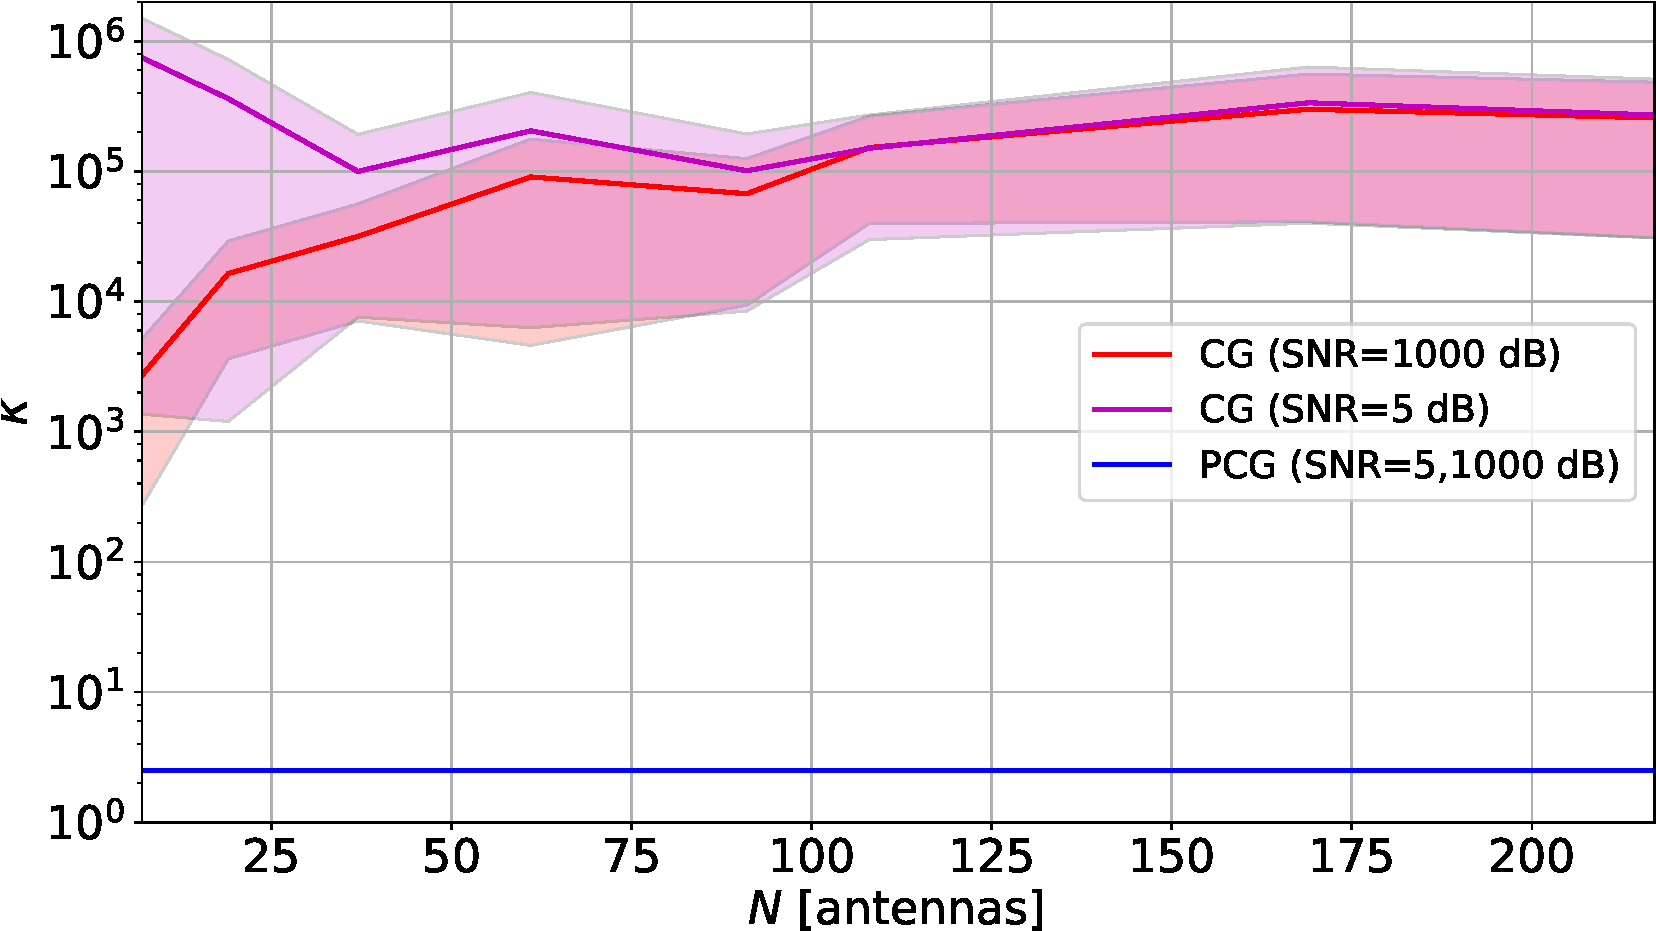
\includegraphics[width=0.47\textwidth]{./kappa.pdf}\label{fig:kappa}}
% V_R_3.pdf: 585x441 pixel, 72dpi, 20.64x15.56 cm, bb=0 0 585 441
\subfigure[Iterations required before and after Preconditioning]{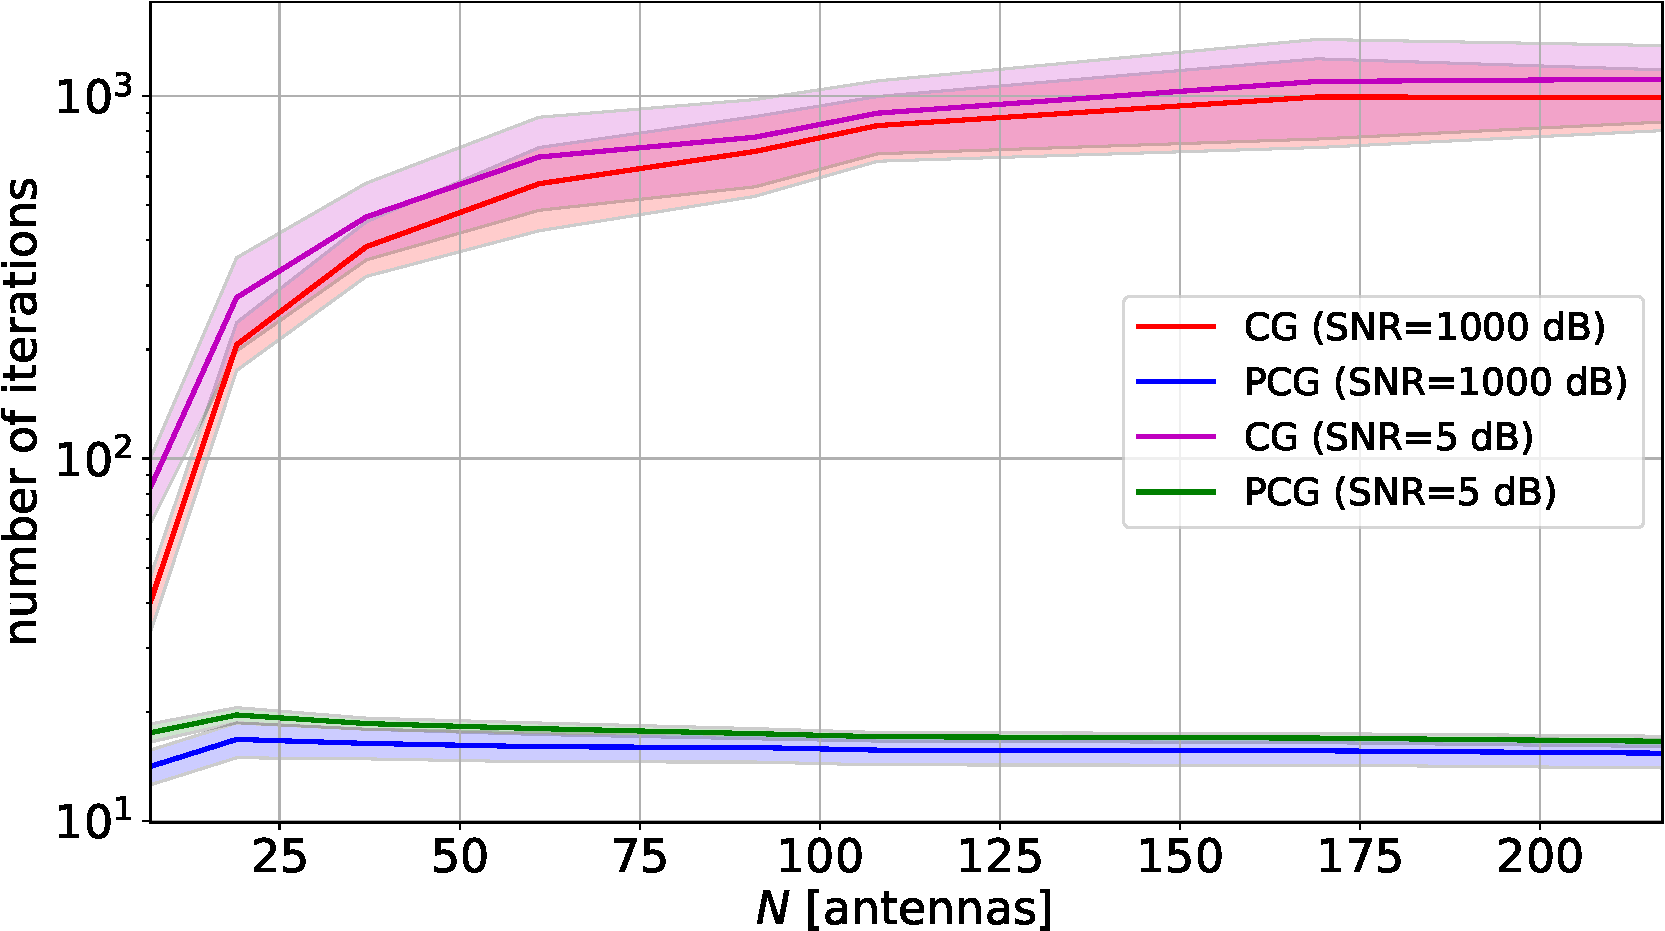
\includegraphics[width=0.47\textwidth]{./cg_itr.pdf}\label{fig:cg_itr}}
\caption{The graphs presented here were generated using the simulations discussed in Section~\ref{sec:red_wirtinger}. Left: spectral condition number $\kappa$ of the modified Hessian $\bmH$ as a function of $N$, before (magenta and red curves) and after (blue curve) preconditioning, at different SNR values. Right: number of major iterations required by the conjugate 
gradient method to invert $\bmH$ as a function of the number of antennas $N$ in the array, before (magenta and red curves) and after preconditioning (blue and green curves), at different SNR values. Both plots show that the Jacobian preconditioner definitely speed up the conjugate gradient method. \label{fig:kappa_itr}} 
\end{figure*}

%The graphs presented here were generated using the second experimental setup in Table~\ref{tab:ch_parm}.

Let us now shift our attention towards the remaining factor $m$. To get a usefull idea of the computational complexity of CG, we must relate $m$ and $P$. This can be achieved by utilizing the modified Hessian's measure of sparsity $\gamma$:   
\begin{equation}
 \gamma = \left (1 - \frac{m}{P^2} \right ),
\end{equation}
where $m$ is the number of non-zero entries in $\bmH$  and $P^2$ is total number of matrix elements.

For a regular east-west geometric configuration the sparsity and the asymptotic sparsity of $\bmH$ can be derived analytically:
\begin{align}
\gamma &= \frac{5N^2-7N+3}{8N^2-8N+2} & \gamma_{\infty} &= \lim_{N\rightarrow \infty}\gamma = \frac{5}{8} \label{eq:gamma}. 
\end{align}
For more complicated array layouts, however, there is no straightforward analytical solution and we empirically determined the sparsity ratios for three different geometric layouts as a function of the number antennas in the array (see Figure~\ref{fig:gamma}). 

It now follows that 
%{\bf (GB: can't follow why it is this way...)}
%{\bf (TLG: Rewrote this to emphasize the link between $m$ and $P$, the computational complexity is only useful, if it is expressed in terms of the number of parameters one whises to solve for. Multiplying the $1-$ sparsity measure with $P^2$ gives you $m$. Moreover,since it is smaller than one, this tells us that we are doing better than $P^2$. The reduction in complexity stems from sparse vector matrix multiplication.)}
\begin{equation}
P^{c} = m = (1 - \gamma)P^2,
\end{equation}
which leads to
\begin{align}
c &= \log_{P}(1 - \gamma) + 2 & c_{\infty} &= \lim_{N\rightarrow \infty} c = 2. \label{eq:c}
\end{align}
The computational complexity is therefore asymptotically bounded by $O(P^2)$, although it converges very slowly to its asymptotic value, and in general is equal to $O(P^{c})$, where $c \sim 1.7$ in the case of an hexagonal geometric layout with $N < 200$ (see Figure~\ref{fig:c}).

\begin{figure*}
\centering
\subfigure[$\gamma$]{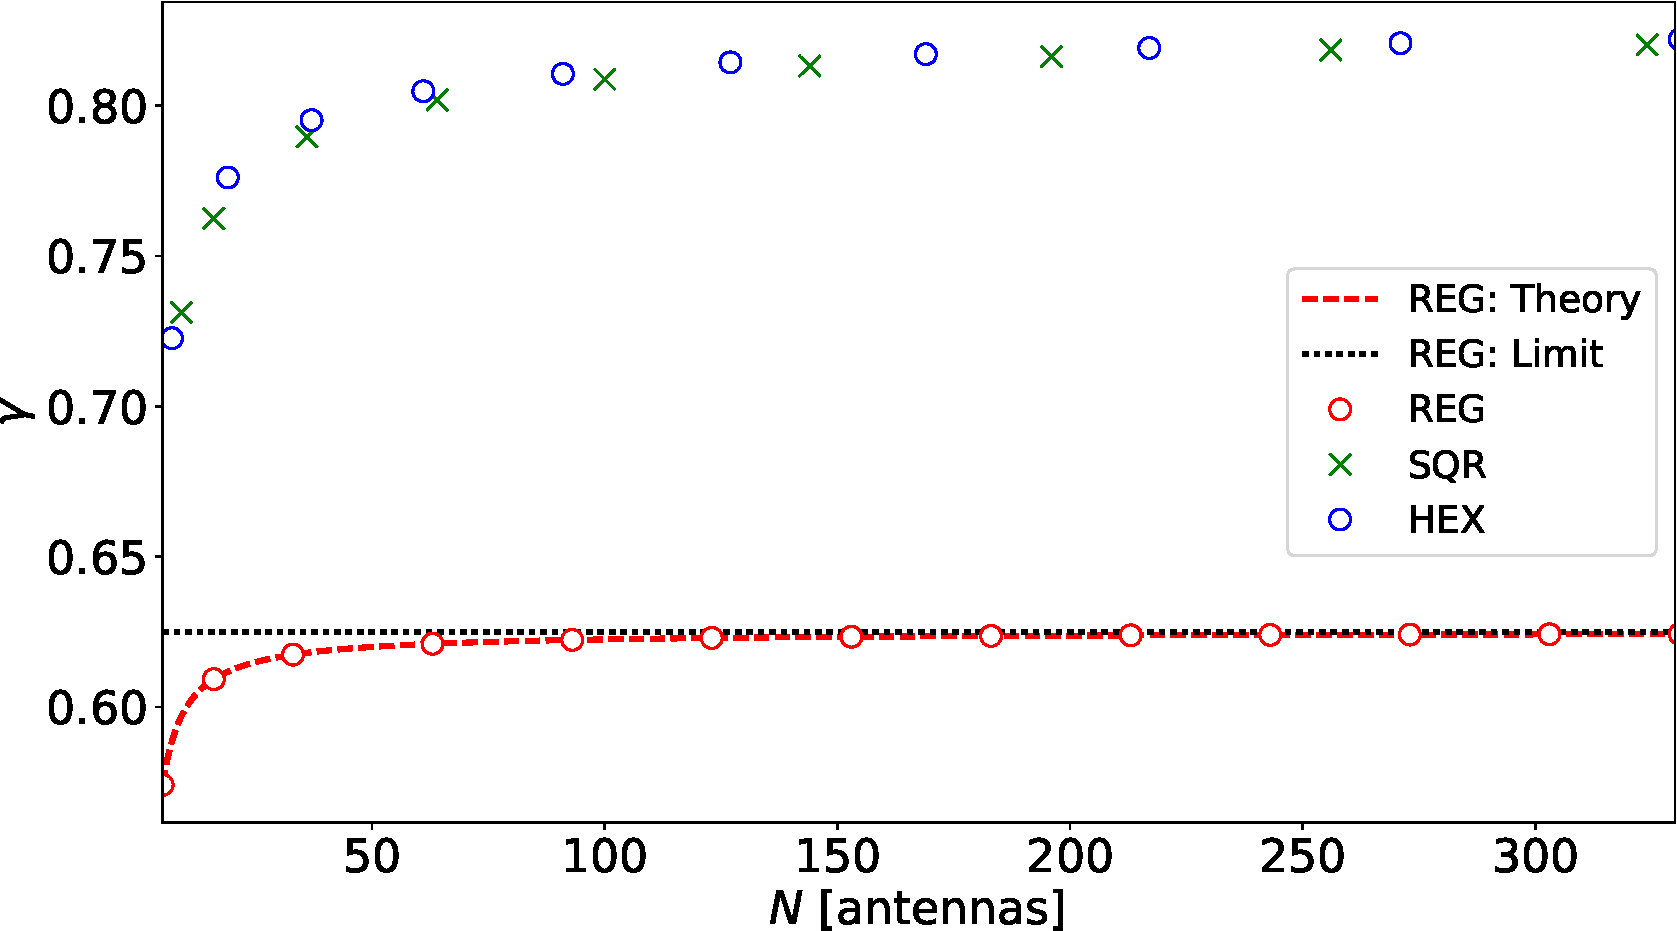
\includegraphics[width=0.47\textwidth]{./sparsity.pdf}\label{fig:gamma}}
% V_R_3.pdf: 585x441 pixel, 72dpi, 20.64x15.56 cm, bb=0 0 585 441
\subfigure[$c$]{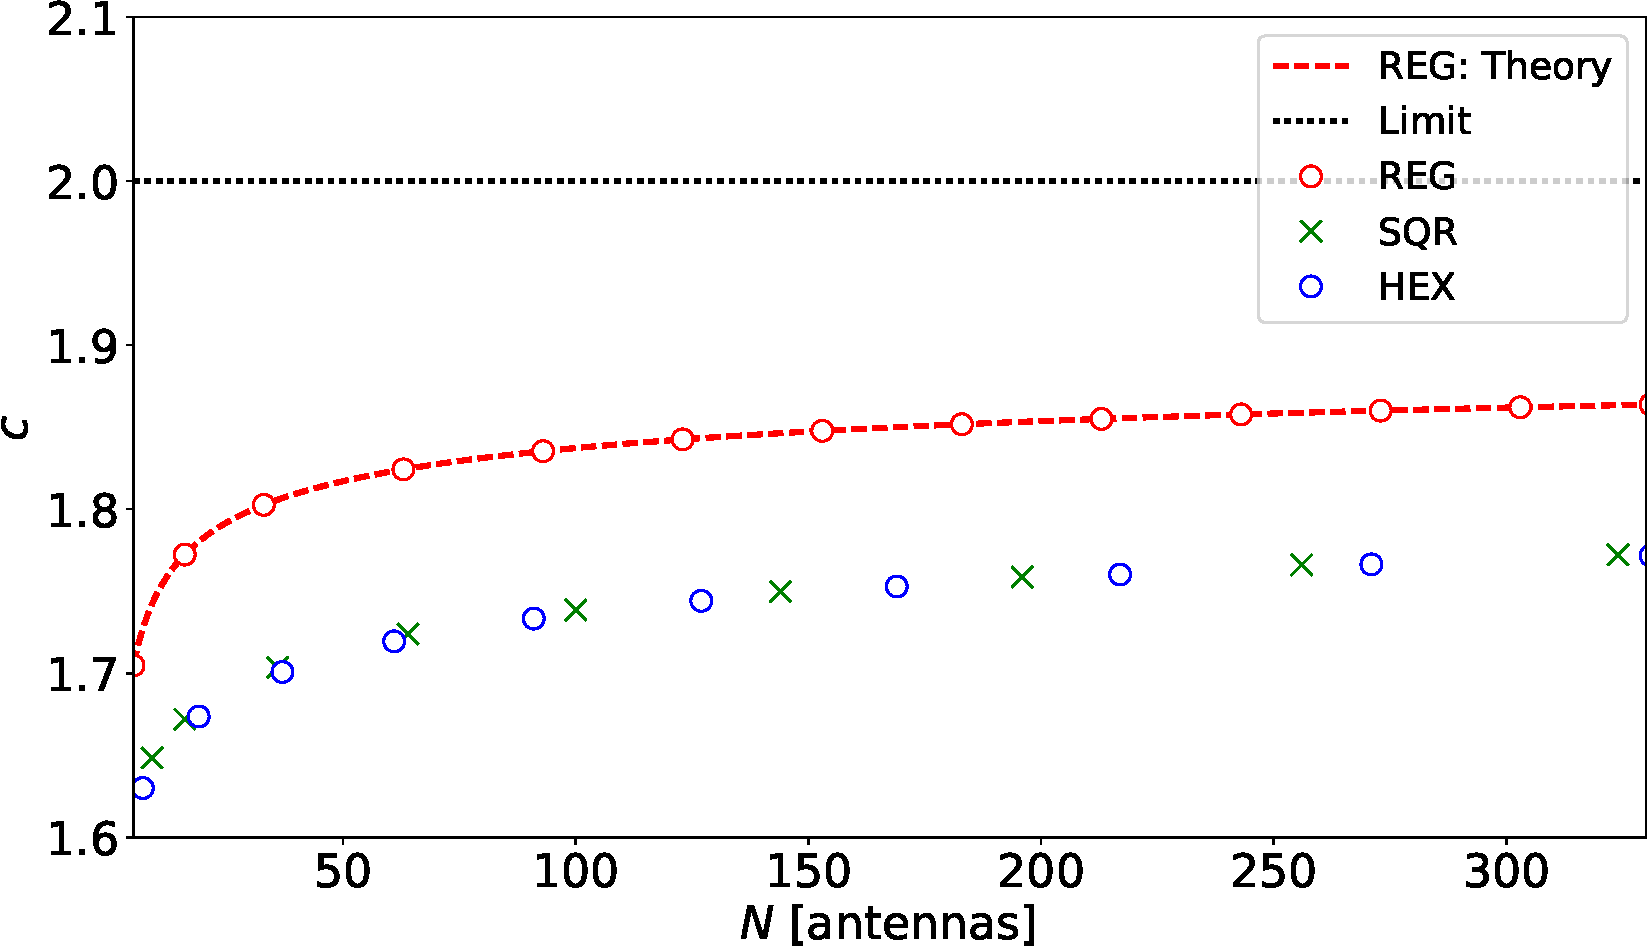
\includegraphics[width=0.46\textwidth]{./comp_order.pdf}\label{fig:c}}
\caption{Left: the sparsity ratio $\gamma$ of the modified Hessian $\bmH$ as a function of the number of antennas $N$ for an hexagonal (blue circles), square (green crosses) and regular east-west (red circles) array geometry. The red--dashed and black--dotted lines show the analytical expression for $\gamma$ and its limit for the regular east-west grid case (see text for details). Right: the order of the computational cost $c$ for inverting $\bmH$ as a function of $N$ for different array geometries (same colour scheme as in the left panel). The red--dashed and black--dotttedlines are the analytical expression of $c$ and its limit in the east-west regular grid case.
\label{fig:sparsity}} 
\end{figure*}

We are now finally able to compare the computational complexity of redundant \textsc{StEfCal} and the PCG method. Redundant \textsc{StEfCal} is computationally inexpensive as it just needs to invert a diagonal matrix, however, the PCG inversion is accurate and, therefore, may require fewer iterations, ultimately leading to a faster convergence. 
We computed the theoretical number of redundant \textsc{StEfCal} iterations $\Delta k$, in excess of the number of LM (implementing PCG) iterations required, for LM to outperform redundant \textsc{StEfCal}
\begin{align}
\label{eq:k} 
 (k+\Delta k)P >& \, kP^c, & \Delta k >& \, k(P^{c-1}-1),
\end{align}
and compared it to the empirically obtained average excess number of iterations. The results are displayed in Figure~\ref{fig:out_diff} which shows that redundant \textsc{StEfCal} outperforms the PCG method. We note that, in this comparison, we have only taken into account the cost of inverting $\bmH$ and ignored the cost of preconditioning. 
%The PCG method is still useful in practice as it would be more straightforward to apply it to other calibration use cases 
%
%{\bf (GB: what do you mean with this statements? Which cases?)}.
%{\bf (TLG: I was hoping that Jonathan would have published his work by now. In it he shows that the pointing error formulation has off-diagonal significant elements. We should prob just remove this sentence as I can not reference anything as of yet.)}

\begin{figure*}
\centering
\subfigure[Number of LM iterations required by redundant \textsc{StEfCal} and PCG.]{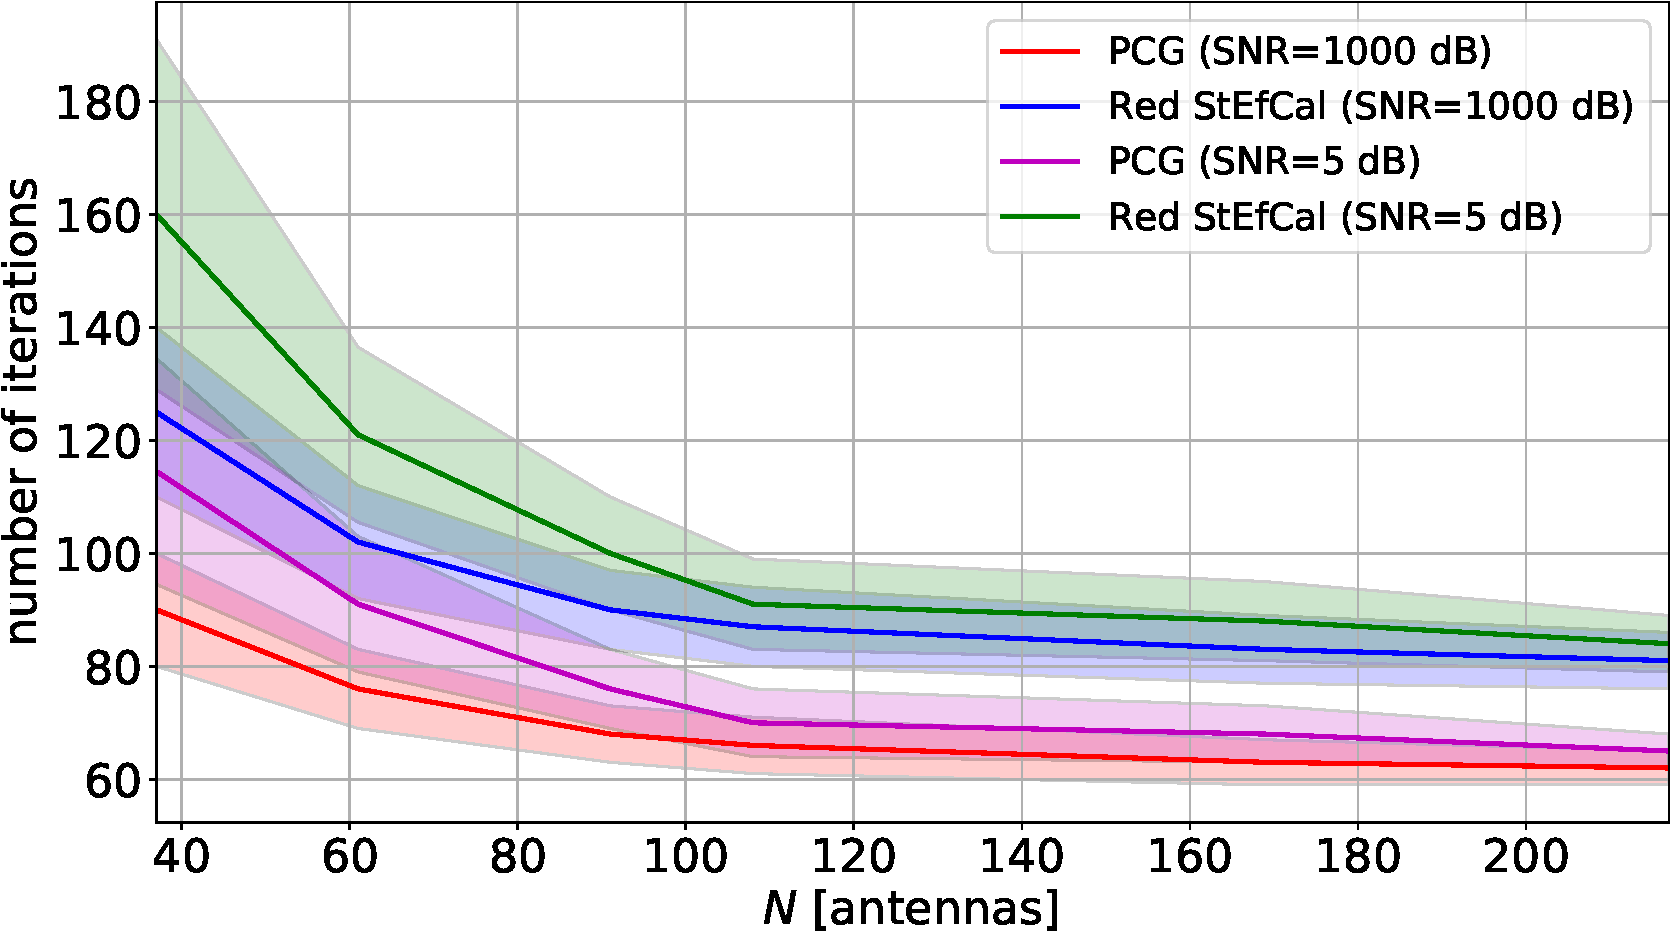
\includegraphics[width=0.45\textwidth]{./outerloop.pdf}\label{fig:outerloop}}
% V_R_3.pdf: 585x441 pixel, 72dpi, 20.64x15.56 cm, bb=0 0 585 441
\subfigure[Difference.]{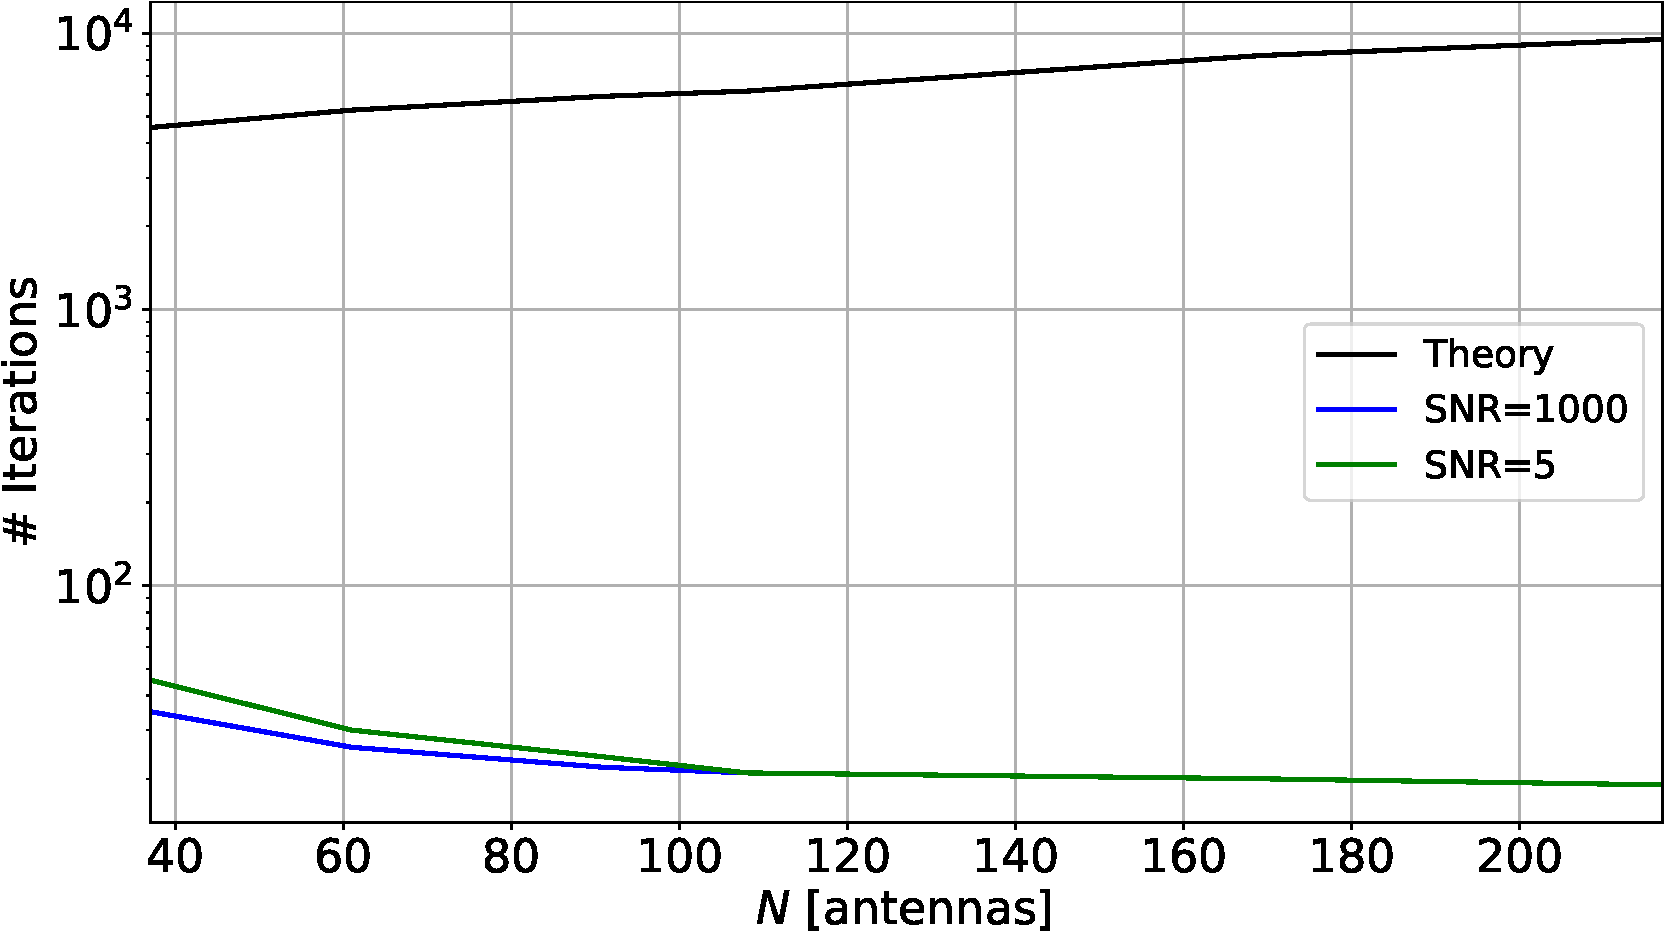
\includegraphics[width=0.45\textwidth]{./diff.pdf}\label{fig:diff}}
\caption{The graphs presented here were generated using the simulations discussed in Section~\ref{sec:red_wirtinger}. Left: number of LM iterations required by redundant \textsc{StEfCal} (green and blue curves) and the PCG (magenta and red curves) methods to converge to a parameter error tolerance of $10^{-6}$ whilst using different SNR values as a function of the number of antennas $N$ in the array. Right: average amount of LM iterations (difference between the redundant \textsc{StEfCal} and PCG curves in the left panel) saved (green and blue curve) by computing the full-inverse with the PCG method whilst using different SNR values. The black curve is $\Delta k$, the theoretical number 
of redundant \textsc{StEfCal} iterations that are needed in excess of the number of LM iterations used for the LM algorithm to 
outperform redundant \textsc{StEfCal}. For the black curve we assumed $c=1.7$ and that $k$ could be approximated with the 
the magenta curve plotted in the left panel.
\label{fig:out_diff}} 
\end{figure*}


\section{Conclusion}
\label{sec:conclusions}
In this paper we have formulated the calibration of redundant interferometric arrays using the complex optimization formalism 
\citep{Smirnov2015}. We derived the associated complex Jacobian and the GN and LM parameter update steps.
We also showed that the LM parameter update step can be simplified to obtain an ADI type of algorithm \citep[][]{Salvini2014,Marthi2014}.
Our code implementation of this algorithm (redundant \textsc{StEfCal}) is publicly available at 
\url{https://github.com/Trienko/heracommissioning/blob/master/code/stef.py}. 
We note that, in its current implementation, redundant \textsc{StEfCal} does not solve for the degeneracies inherent to redundant calibration  \citep{Zheng2014,Kurien2016} which will be the subject of future work. Compared to current redundant calibration algorithms, redundant \textsc{StEfCal} is more robust to inital conditions and allows for an easier, massive parallelization. 

We investigated the computational cost of redundant \textsc{StEfCal} and compared it with the performance of the PCG method (approach suggested by \cite{Liu2010}).
We found that, although the PCG method method greatly improves the speed of redundant calibration, it still significant underperforms in comparison to redundant \textsc{StEfCal}.

The characteristics of redundant \textsc{StEfCal} make it an appealing calibration algorithm for large redundant arrays like HERA \citep{deboer2017}, CHIME \citep{Bandura2014}, HIRAX \citep{Newburgh2016} or even hybrid arrays like the MWA \citep{Tingay2013} in its updated phase.

\section*{Acknowledgements}
G.B. acknowledges support from the Royal Society and the Newton Fund under grant NA150184. This work is based on the research supported in part by the National Research Foundation of South Africa (grant No. 103424). This research is supported by the South African Research Chairs Initiative of the Department of Science and Technology and National Research Foundation,



\bibliographystyle{mn2e}
\bibliography{paper}

\appendix

{\bf (GB: We need to bring back the logcal and lincal derivation using the geometric function.)}
%{\bf (TLG: I have removed logcal and lincal as well as the PCG section. My main concern about this is that the aim of these sections was to show off the usefulness of the geometry function, it simplifies, at least from a mathematecial perspective, the derivation of the older algorithms. This insight has now been lost. On the other hand keeping them and trying to make them fit, which may cause further delays, at this point simply no longer seems worht the effort. I have incorporated the remaining ideas left in the PCG section into the main text.)}.
%
% \section{\textsc{LOGCAL}}
% \label{sec:logcal}
% We can rewrite equation~\ref{eq:vis_red} to \citep{Liu2010}
% \begin{eqnarray}
% \ln |d_{pq}| &=& \ln |g_p| + \ln |g_q| + \ln |y_{\phi_{pq}}| + s_{pq} \label{eq:logcal_amp}\\
% \angle d_{pq} &=& \angle g_p - \angle g_q + \angle \phi_{pq} + t_{pq} \label{eq:logcal_phase}
% \end{eqnarray}
% where
% \begin{align}
% s_{pq} &= \mathscr{R} \left \{1 + \frac{n_{pq}}{g_p\conj{g_q}y_{\phi_{pq}}} \right \}, & t_{pq} &= \mathscr{I}\left \{1 + \frac{n_{pq}}{g_p\conj{g_q}y_{\phi_{pq}}} \right \}.
% \end{align}
% Moreover, $\mathscr{R}\{*\}$ and $\mathscr{I}\{*\}$ denote the real and imaginary operators. 
% 
% With the aid of equation~\ref{eq:logcal_amp} we can construct the following linear system:
% \begin{equation}
% \label{eq:log_system}
% \bdelta = \bJ\bzeta + \bs, 
% \end{equation}
% where
% \begin{align}
% \left [ \bdelta \right ]_{\alpha_{pq}} &= \ln |d_{pq}|, & \left [ \bs \right ]_{\alpha_{pq}} = s_{pq} 
% \end{align}
% and
% \begin{equation}
% \left [ \bzeta \right ]_{j} = \begin{cases} \ln |g_j| & \textrm{if}~j\leq N \\ \ln |y_{j-N}| & \textrm{otherwise} \end{cases}. 
% \end{equation}
% Furthermore,
% \begin{equation}
% \bJ = 
% \begin{bmatrix}
% \bN & \bM
% \end{bmatrix}
% \end{equation}
% with 
% \begin{equation}
% [\bN]_{\alpha_{pq},j} = \begin{cases}
%        1 & \textrm{if}~(p=j)~\textrm{or}~(q=j)\\
%        0 & \textrm{otherwise}
%       \end{cases}
% \end{equation}
% and
% \begin{equation}
% [\bM]_{\alpha_{pq},j} = \begin{cases}
%        1 & \textrm{if}~\phi_{pq}=j\\
%        0 & \textrm{otherwise}
%       \end{cases}
% \end{equation}
% 
% The least squares solution to Eq.\ref{eq:log_system}, under the incorrect assumption that $s_{pq}$ is normally distributed, is given by
% \begin{equation}
% \bzeta = (\bA^T\bA)^{-1} \bA^T\bdelta. 
% \end{equation}
% How to correctly deal with the fact that $s_{pq}$ is not normally distributed is discussed in \citep{Liu2010}. A similar linear system can be constructed for equation~\ref{eq:logcal_phase}. 
% From the least squares solutions to the linear systems associated with equation~\ref{eq:logcal_amp} and equation~\ref{eq:logcal_phase} we can compute the antenna gains as well as the true visibilities.
% 
% \section{\textsc{lincal}}
% \label{sec:lincal}
% Assume that $\eta_p,\eta_q,\widetilde{\eta}_{\phi_{pq}},\varphi_p,\varphi_q$ and $\widetilde{\varphi}_{\phi_{pq}}$ are real valued variables.
% We can rewrite equation~\ref{eq:vis_red_vec} to \citep{Liu2010}
% \begin{equation}
% \label{eq:lincal_vec}
% \bd = \bv(\bvarrho) + \bn, 
% \end{equation}
% where 
% \begin{align}
% \left [ \bv(\bvarrho) \right ]_{\alpha_{pq}} &= e^{\eta_p - i \varphi_p} e^{\widetilde{\eta}_{\phi_{pq}}- i \widetilde{\varphi}_{\phi_{pq}}} e^{\eta_q + i \varphi_q}\\
% &= v_{pq},
% \end{align}
% and
% \begin{equation}
% \bvarrho = 
% \begin{bmatrix}
% \bmath{\eta} \\
% \bvarphi \\
% \widetilde{\bmath{\eta}} \\
% \widetilde{\bvarphi}
% \end{bmatrix},\qquad
% \begin{aligned}
% \bmath{\eta} &= [\eta_1, \eta_2,\cdots \eta_N]^T\\
%  \bmath{\varphi} &= [\varphi_1, \varphi_2,\cdots \varphi_N]^T\\
%  \widetilde{\bmath{\eta}} &= [\widetilde{\eta}_1, \widetilde{\eta}_2,\cdots \widetilde{\eta}_L]^T\\
%  \widetilde{\bmath{\varphi}} &= [\widetilde{\varphi}_1, \widetilde{\varphi}_2,\cdots \widetilde{\varphi}_L]^T
% \end{aligned}.
% \label{eq:help}
% \end{equation}
% Note that the vectors $\bmath{\eta},~\bvarphi,~\widetilde{\bmath{\eta}}$ and $\widetilde{\bvarphi}$ are real valued.
% 
% The first order Taylor expansion of equation~\ref{eq:lincal_vec} around the fiducial point $\bvarrho_0$ is equal to
% \begin{equation}
% \label{eq:d_lin}
% \bd = \bv_0 + \bmJ_0 \Delta \bvarrho  + \bn.
% \end{equation}
% If we calculate the residual, dropping the reference to a specific fiducial point, we obtain: 
% \begin{equation}
% \label{eq:r_lin}
% \br = \bd - \bv = \bmJ \Delta \bvarrho + \bn.
% \end{equation}
% Moreover,
% \begin{equation}
% \label{eq:jac_upper_lincal}
% \bmJ = \begin{bmatrix}
%        \bN & \bM 
%        \end{bmatrix},
% \end{equation}
% where
% \begin{align}
% \bN &= \begin{bmatrix} \bO & \bP \end{bmatrix}, & \bM &= \begin{bmatrix} \bQ & \bR \end{bmatrix}, 
% \end{align}
% \begin{equation}
%  [\bO]_{\alpha_{pq},j} =  \frac{\partial v_{pq}}{\partial \eta_j} = \begin{cases} 
%     v_{pq} &\textrm{if}~(p=j)~\textrm{or}~(q=j)\\
%     0 & \textrm{otherwise}
%    \end{cases},
% \end{equation}
% \begin{equation}
%  [\bP]_{\alpha_{pq},j} =  \frac{\partial v_{pq}}{\partial \varphi_j} = \begin{cases}
%                                                                         i v_{pq} &\textrm{if}~ p=j\\
%                                                                         -i v_{pq} &\textrm{if}~ q=j \\
%                                                                         0 & \textrm{otherwise} 
%                                                                        \end{cases}
% \end{equation}
% \begin{equation}
%  [\bQ]_{\alpha_{pq},j} =  \frac{\partial v_{pq}}{\partial \widetilde{\eta}_j} = \begin{cases} 
%     v_{pq} &\textrm{if}~\phi_{pq}=j\\
%     0 & \textrm{otherwise}
%    \end{cases},
% \end{equation}
% \begin{equation}
%  [\bR]_{\alpha_{pq},j} =  \frac{\partial v_{pq}}{\partial \widetilde{\varphi}_j} = \begin{cases} 
%     i v_{pq} &\textrm{if}~\phi_{pq}=j\\
%     0 & \textrm{otherwise}
%    \end{cases}.
% \end{equation}
% Augmenting the residual by taking into account its conjugate results in 
% \begin{equation}
% \breve{\br} = \bJ \Delta \bvarrho + \bn, 
% \end{equation}
% where $\breve{\br} = \begin{bmatrix}\br^T & \conj{\br}^T \end{bmatrix}^T$ and 
% \begin{equation}
% \label{eq:Jac_lin}
% \bJ = 
% \begin{bmatrix}
%  \bmJ\\  
%  \conj{\bmJ}
% \end{bmatrix}.
% \end{equation}
% The solution to 
% \begin{equation}
%  \min_{\Delta \bvarrho} \| \breve{\br} - \bJ \Delta \bvarrho\|_F^2,
% \end{equation}
% is equal to 
% \begin{equation}
% \label{eq:LINCAL_update}
% \Delta \bvarrho = (\bJ^H\bJ)^{-1} \bJ^H\breve{\br}. 
% \end{equation}
% equation~\ref{eq:LINCAL_update} is used to iteratively determine a new estimate of the parameter vector $\bvarrho$ as follows
% \begin{equation}
% \label{eq:new_rho}
% \bvarrho_{k+1} = \bvarrho_k + \Delta \bvarrho_k. 
% \end{equation}
% Note that we do not explicitly denote the $k$ index in equation~\ref{eq:LINCAL_update}.
% Moreover, equation~\ref{eq:LINCAL_update} is the GN update associated with the following minimization problem \citep{Kurien2016}
% \begin{equation}
% \label{eq:least_squares_lincal}
% \min_{\bmath{\varrho}} \|\breve{\br}\| = \min_{\bmath{\varrho}} \|\breve{\bd} - \breve{\bv}(\bmath{\varrho})\|.
% \end{equation}

% \section{Conjugate Gradient Method}
% 
% \subsection{Normal Equation}
% \label{sec:normal}
% Lets assume that instead of equation~\ref{eq:linear_system} we have a more general linear system, i.e.
% \begin{equation}
%  \bb = \bB\bx,
% \end{equation}
% where $\bb\in\mathbb{C}^K$, $\bx\in\mathbb{C}^P$  and $\bB\in\mathbb{C}^{K \times P}$, with $K > P$. We can use the normal equation 
% \begin{equation}
% \label{eq:normal_equation}
% \bB^H\bB\bx = \bB^H\bb, 
% \end{equation}
% to estimate the $\bx$ that minimizes
% \begin{equation}
% \label{eq:norm_ls}
% \|\bb-\bB\bx\|_F^2. 
% \end{equation}
% In this paper, we denote the Hermitian transpose with $(*)^H$ and the Frobenius norm with $\|*\|_F$.
% 
% There are a few important observations that we can make while inspecting equation~\ref{eq:normal_equation}:
% \begin{enumerate}
% \item $\bB^H\bB$ is a square positive semi-definite Hermitian matrix by construction.
% \item $\bB^H\bb$ is in the column range of $\bB^H\bB$; this follows trivially from 
% \begin{equation}
% \bB^H\bb \in \mathcal{R}(\bB^H) \implies \bB^H\bb \in \mathcal{R}(\bB^H\bB).   
% \end{equation}
% \end{enumerate}
% In this paper, we denote the column range of a matrix $\bA$ with $\mathcal{R}(\bA)$.
% 
% Recall that we mentioned that in general we can only solve equation~\ref{eq:linear_system} with CG if $\bA$ is a square positive-definite Hermitian matrix. The CG method actually has an even broader applicability: it can be used to solve equation~\ref{eq:linear_system} even if $\bA$ is a Hermitian positive semi-definite
% square matrix as long as $\bb$ is in the column range of $\bA$ \citep{Lu2015}. In light of \citet{Lu2015}, the two observations in the numbered list we presented in the previous paragraph imply that equation~\ref{eq:normal_equation}
% can be solved by employing the CG method. The solution returned by CG is, however, only unique if $\bB^H\bB$ is positive-definite (invertible). The solution
% obtained by CG, whether it is unique or not, does minimize equation~\ref{eq:norm_ls} in a least squares sense.
% 
% Note that if $\bA$ is positive semi-definite, its smallest eigenvalue is zero. This implies that equation~\ref{eq:kappa} is not defined. \citet{Lu2015} show that when $\bA$
% is a square positive semi-definite Hermitian matrix we do not use the spectral condition number to bound the convergence complexity of CG, but the general spectral condition
% number instead. The general spectral condition number is very similar to the spectral condition number; the only difference being that in equation~\ref{eq:kappa} we replace  
% $\lambda_{\textrm{min}}$ with $\lambda_{\textrm{min}}^+$, which denotes the smallest positive eigenvalue.

\section{Derivation of redundant Wirtinger calibration}
\label{sec:analytic}
If we apply the definition in equation~\ref{eq:Jacobian} to equation~\ref{eq:least_squares_complex} we obtain the following analytic result:
\begin{equation}
\label{eq:Jacobian_red}
\bJ = \begin{bmatrix}
       \bM & \bN\\
       \conj{\bN} & \conj{\bM}
      \end{bmatrix},
\end{equation}
where
\begin{equation}
\bM =\begin{bmatrix}
      \bO & \bP
     \end{bmatrix},
\end{equation}
and 
\begin{equation}
\bN = \begin{bmatrix}
       \bQ & \bzero
      \end{bmatrix}.
\end{equation}
Moreover,
\begin{equation}
\left [ \bO  \right ]_{\alpha_{pq},j} = \begin{cases}
                                         y_{\phi_{pq}}\conj{g_q} & \textrm{if}~p=j\\
                                         0  & \textrm{otherwise} 
                                        \end{cases},
\end{equation}

\begin{equation}
\left [ \bP  \right ]_{\alpha_{pq},j} = \begin{cases}
                                         g_p\conj{g_q} & \textrm{if}~\phi_{pq}=j\\
                                         0  & \textrm{otherwise} 
                                        \end{cases}
\end{equation}
and
\begin{equation}
\left [ \bQ  \right ]_{\alpha_{pq},j} = \begin{cases}
                                         g_py_{\phi_{pq}} & \textrm{if}~q=j\\
                                         0  & \textrm{otherwise} 
                                        \end{cases}
\end{equation}

We use $\bzero$ to denote an all zero matrix. It is now trivial to compute the Hessian $\bH$ by using equation~\ref{eq:Jacobian_red}. If we substitute equation~\ref{eq:Jacobian_red} into $\bJ^H\bJ$
we obtain 
\begin{equation}
\label{eq:red_H}
\bH = \bJ^H\bJ = 
\begin{bmatrix}
\bA & \bB\\
\conj{\bB} & \conj{\bA}
\end{bmatrix},
\end{equation}
where

\begin{align}
\bA &= \begin{bmatrix} \bC & \bD\\ \bD^H & \bE \end{bmatrix}, & \bB &= \begin{bmatrix} \bF & \bG\\ \bG^T & \bzero \end{bmatrix},
\end{align}

\begin{equation}
[\bC]_{ij} = 
\begin{cases}
 \sum_{k \neq i} \left | g_k \right |^2 \left | y_{\zeta_{ik}} \right |^2 & \textrm{if} ~ i=j\\
 0 & \textrm{otherwise}
\end{cases},
\end{equation}
\begin{equation}
[\bD]_{ij} = 
\begin{cases}
 g_i \conj{y}_j  \left | g_{\psi_{ij}} \right |^2  & \textrm{if} ~ \psi_{ij}\neq0\\
 0 & \textrm{otherwise}
\end{cases},
\end{equation}

\begin{equation}
[\bE]_{ij} = 
\begin{cases}
 \sum_{rs \in \mathcal{RS}_i} \left | g_r \right |^2 \left | g_s \right |^2  & \textrm{if} ~ i=j\\
 0 & \textrm{otherwise}
\end{cases},
\end{equation}
\begin{equation}
[\bF]_{ij} = 
\begin{cases}
 g_i g_j  \left | y_{\zeta_{ij}} \right |^2  & \textrm{if} ~ i \neq j\\
 0 & \textrm{otherwise}
\end{cases},
\end{equation}
and
\begin{equation}
[\boldsymbol{G}]_{ij} = 
\begin{cases}
 g_i y_j  \left | g_{\xi_{ij}} \right |^2  & \textrm{if} ~ \xi_{ij}\neq0\\
 0 & \textrm{otherwise}
\end{cases}.
\end{equation}
Moreover, 
\begin{equation}
\label{eq:RS}
\mathcal{RS}_i = \left\{rs\in\mathbb{N}^2|(\phi_{rs} = i) \right\},
\end{equation}
\begin{equation}
\xi_{ij} = 
\begin{cases}
p~\textrm{if}~\exists! ~ p \in \mathbb{N} ~ s.t. ~(\phi_{pi} = j)\\
0~\textrm{otherwise}
\end{cases},
\end{equation}
and
\begin{equation}
\psi_{ij} = 
\begin{cases}
q~\textrm{if}~\exists! ~ q \in \mathbb{N} ~ s.t. ~(\phi_{iq} = j)\\
0~\textrm{otherwise}
\end{cases}.
\end{equation}

Furthermore, substituting equation~\ref{eq:Jacobian_red} into $\bJ^H\breve{\br}$ results in
\begin{equation}
\bJ^H\breve{\br} = \begin{bmatrix}
                   \ba \\
                   \bb \\
                   \conj{\ba}\\
                   \conj{\bb}
                   \end{bmatrix},
\end{equation}
where
\begin{align}
\label{eq:ab}
\left [ \ba \right ]_i &= \sum_{k\neq i} g_k \widetilde{y}_{ik}r_{ik},  & \left [ \bb \right ]_i &= \sum_{rs\in\mathcal{RS}_i}\conj{g}_r g_s r_{rs},
\end{align}
and
\begin{equation}
\label{eq:y_tilde}
\widetilde{y}_{ik} = 
\begin{cases}
\conj{y}_{\zeta_{ik}} & \textrm{if}~k > i\\
y_{\zeta_{ik}} & \textrm{otherwise}
\end{cases}.
\end{equation}
Additionally, $\ba$ and $\bb$ are both column vectors. The lengths of $\ba$ and $\bb$ are $N$ and $L$ respectively.
The dimensions of the matrices we defined in this section are presented in Table~\ref{tab:matrix_dimensions}.

Furthermore,
\begin{align}
\label{eq:identities}
\frac{1}{3}\bJ\breve{\bz} &= \breve{\bv}, & \bJ^H\breve{\bv} &= (\bI\odot\bH)\breve{\bz} 
\end{align}
The above identities can be trivially established by mechanically showing that the left hand side of each expression in equation~\ref{eq:identities} is equal to its right hand side.
In equation~\ref{eq:identities}.

\begin{table}
\centering
\caption{The dimensions of the matrices defined in Appendix~\ref{sec:analytic}.}
\begin{tabular}{|c c|} 
\hline
Matrix & Dimension\\
\hline
\hline
$\bJ$ & $2B \times P$ \\
$\bM$ & $B \times (N+L)$ \\
$\bN$ & $B \times (N+L)$ \\
$\bO$ & $B \times N$ \\
$\bP$ & $B \times L$ \\
$\bQ$ & $B \times N$ \\
$\bzero$ & $B \times L$ \\
\hline
\hline
$\bH$ & $P\times P$\\
$\bA$ & $(N+L)\times (N+L)$\\
$\bB$ & $(N+L)\times (N+L)$\\
$\bC$ & $N \times N$\\
$\bD$ & $N \times L$\\
$\bE$ & $L \times L$\\
$\bF$ & $N \times N$\\
$\bG$ & $N \times L$\\
$\bzero$ & $L \times L$\\
\hline
\end{tabular}
\label{tab:matrix_dimensions}
\end{table}

\section{ADI}
\label{sec:red_stef_ADI}
The basic skymodel-based \textsc{StEfCal} update step is equal to  the leftmost term in equation~\ref{eq:g_update} (barring $\alpha$) \citep{Salvini2014}.
Assume without any loss of generality that the array is in an east-west regular grid. Furthermore, assume that $\boldsymbol{d}$ (see equation~\ref{eq:vis_linear_definition}) has been re-ordered 
and that the result of this re-ordering is the following
\begin{equation}
\widetilde{\boldsymbol{d}} = \left[d{12},\cdots,d_{N-1,N},d_{13},\cdots,d_{N-2,N},\cdots,d_{1N}\right]^T .
\end{equation}
The vector $\widetilde{\bn}$ should be interpreted in a similar manner.

Equation~\ref{eq:vis_linear_definition} can now be rewritten as 
\begin{equation}
\label{eq:linear_system}
\widetilde{\boldsymbol{d}} = \boldsymbol{J}\boldsymbol{y} + \widetilde{\bn}, 
\end{equation}
if we assume that $\boldsymbol{g}$ and its conjugate are known vectors. In equation~\ref{eq:linear_system},
\begin{equation}
\boldsymbol{J} = 
\begin{bmatrix}
g_1\conj{g}_2 & 0 & \cdots & 0\\
g_2\conj{g}_3 & 0 & \cdots & 0\\
\vdots & 0 & \cdots & 0\\
g_{N-1}\conj{g}_N & 0 & \cdots & 0\\
0 & g_1\conj{g}_3 & \cdots & 0\\
0 & \vdots & \cdots & 0\\
0 & g_{N-2}\conj{g}_N & \cdots & 0\\
0 & 0 & \cdots & 0\\
  & \vdots & \\
0 & 0 & \cdots & g_1\conj{g}_N\\  
\end{bmatrix}.
\end{equation}
We can now estimate $\boldsymbol{y}$ with
\begin{equation}
\label{eq:y_final}
\boldsymbol{y} = (\boldsymbol{J}^H\boldsymbol{J})^{-1}\boldsymbol{J}^H\widetilde{\boldsymbol{d}}, 
\end{equation}
where 
\begin{equation}
\label{eq:RHR}
[\boldsymbol{J}^H\boldsymbol{J}]_{ij} = 
\begin{cases}
\sum_{rs\in\mathcal{RS}_i} |g_r|^2|g_s|^2 &\textrm{if}~i=j\\
0&\textrm{otherwise}
\end{cases},
\end{equation}
and
\begin{equation}
\label{eq:RHd}
[\boldsymbol{J}^H\widetilde{\boldsymbol{d}}]_i = \sum_{rs\in\mathcal{RS}_i} \conj{g}_r g_s d_{rs}. 
\end{equation}
Substituting equation~\ref{eq:RHR} and equation~\ref{eq:RHd} into equation~\ref{eq:y_final} and simplifying the result leads to the leftmost term in equation~\ref{eq:y_update} (if we bar $\alpha$ and consider 
only the $i$-th entry of $\by$).
\label{lastpage}
\end{document}


